% \LaTeX-Main\
% !TeX encoding=UTF-8
% !TeX spellcheck=en_US
%%
%% The LaTeX package mercatormap - version 1.2.0 (2024/08/05)
%% mercatormap.tex: Manual
%%
%% -------------------------------------------------------------------------------------------
%% Copyright (c) 2020-2024 by Prof. Dr. Dr. Thomas F. Sturm <thomas dot sturm at unibw dot de>
%% -------------------------------------------------------------------------------------------
%%
%% This work may be distributed and/or modified under the
%% conditions of the LaTeX Project Public License, either version 1.3
%% of this license or (at your option) any later version.
%% The latest version of this license is in
%%   http://www.latex-project.org/lppl.txt
%% and version 1.3 or later is part of all distributions of LaTeX
%% version 2005/12/01 or later.
%%
%% This work has the LPPL maintenance status `author-maintained'.
%%
%% This work consists of all files listed in README
%%
% arara: pdflatex: { shell: yes }
% arara: biber
% arara: pdflatex: { shell: yes }
% arara: pdflatex: { shell: yes }
% arara: pdflatex: { shell: yes, synctex: yes }
\documentclass[a4paper,11pt]{ltxdoc}
\usepackage{mercatormap.doc}

% The following personal API-keys are needed for compilation
% \mrcsetapikey{thunderforest}{YOUR-API-KEY}     % registered key

\def\version{1.2.0}%
\def\datum{2024/08/05}%

\mrcactivatescript% activates Python script

\addbibresource{mercatormap.bib}

\hypersetup{
  pdftitle={Manual for the mercatormap package},
  pdfauthor={Thomas F. Sturm},
  pdfsubject={Map drawing based on pixel map tiles with mercator projection},
  pdfkeywords={map tiles, mercator projection, map drawing}
}

\makeindex

\usetikzlibrary{external}
\tikzsetexternalprefix{_figures/}
\tikzexternalize
\tikzexternaldisable% for final version
\tcbset{shield externalize}

\nocite{Sturm:2020,package:tikz,package:siunitx}

\ExplSyntaxOn
\cs_if_exist:NT \pdfsuppresswarningpagegroup
  {
    \pdfsuppresswarningpagegroup=1
  }
\ExplSyntaxOff

%\includeonly{mercatormap.doc.intro}
%\includeonly{mercatormap.doc.examples}
%\includeonly{mercatormap.doc.definition}
%\includeonly{mercatormap.doc.maptiles}
%\includeonly{mercatormap.doc.drawing}
%\includeonly{mercatormap.doc.scales}
%\includeonly{mercatormap.doc.marker}
%\includeonly{mercatormap.doc.routes}
%\includeonly{mercatormap.doc.orthodromes}
%\includeonly{mercatormap.doc.animations}
%\includeonly{mercatormap.doc.limitations}

%%%%%%%%%%%%%%%%%%%%%%%%%%%%%%%%%%%%%%%%%%%%%%%%%
\begin{document}

\input{mercatormap.doc.abstract.tex}
% !TeX root = mercatormap.tex
% !TeX encoding=UTF-8
% !TeX spellcheck=en_US
% include file of mercatormap.tex (manual of the LaTeX package mercatormap)
\clearpage
\section{Introduction}%

The \texttt{mercatormap} package enables map drawing with the
Web Mercator projection. This is done as an extension to
\tikzname\ \cite{package:tikz} with is complemented by a map
coordinate system and many additional commands and options to add elements
like markers, geodetic networks, bar scales, routes, orthodrome
pieces, distance calculations, etc. Also, the seamless integration of graphics
from public map tile servers is provided through a Python script.

If you are interested in the mathematical background of the Web Mercator projection
and the algorithms of this packages, you are invited to read
\enquote{\fullcite{Sturm:2020}}.

With very few exceptions, the package is programmed with the
|expl3| programming interface for \LaTeX3 \cite{l3kernel:interfaces}.

\medskip


\tikzsetnextfilename{intro_example}%
\begin{tikzpicture}
  \mrcmap[
      type=reference,
      position=48.1579577:11.4980376,
      align=west,
      flex reference scale=20000,
      tex width=\linewidth,
      tex height=5cm,
      source=topplusopen web
    ]{intro_example}
  \mrcdrawmap
  \node[below,font=\fontsize{7pt}{7pt}\sffamily] at (mrcmap.south) {\mrcmapattribution};
  \node[above right, font=\sffamily\footnotesize] at (mrcmap.north west) {\mrcprettymapscale};
  \mrcdrawscalebar[width-in-meter=800,partitions=8,north-east-outside=5mm;1.5mm,
    major style={black!75}]
  \path[every node/.style={above,inner sep=0.5mm,font=\sffamily\tiny}]
    (mrcscalebar.north west) -- (mrcscalebar.north east)
    node[pos=0]{0} node[pos=0.25]{200} node[pos=0.5]{400} node[pos=0.75]{600}
    node[pos=1]{800} node[pos=1,right,yshift=-1mm]{m};
  \mrcdrawnetwork
  \mrcmarker{type=pin, draw=Blue_Gray, fill=Blue_Gray!10, font=\sffamily\footnotesize,
    position=48.1582513:11.5032997, contents={Nymphenburg}}
  \mrcclipmap
  \draw (mrcmap.south west) rectangle (mrcmap.north east);
\end{tikzpicture}



%-------------------------------------------------------------------------------
\subsection{Quick Start}

The package is accompanied with a Python script. You should read
\Fullref{sec:python} for the Python preparations.
The package can be used in three ways:
\begin{itemize}
\item Completely without the Python script.
  This is not recommended, because the usage will be quite restricted.
\item With Python script, but without map tile download.
  There is no usage restriction, but you have to create all content yourself.
  To prevent map tile download, set
  \begin{dispListing}
  \mermapset{supply/target=none}
  \end{dispListing}
\item With Python script and map tile download.
  You need permission and access to a map tile server.
  \Fullref{sec:maptileserver} lists a selection of servers with free
  access (some require registration of an API key).
\end{itemize}

After Python is prepared, you may try to compile
|mercatormap-example.tex| (found in the documentation directory)
which contains a map of Bavaria with map tile download.
\Fullref{sec:examples} exhibits further examples which may serve as
tutorials what can be done. After the examples you find the reference
manual for the package.

\clearpage
%-------------------------------------------------------------------------------
\subsection{Installation of Python and Packages}\label{sec:python}

A Python~3 script is part of the |mercatormap| package.
The main purpose of this script is to download selected map tiles for
the maps of the document. Also, some coordinate system computation is
done by this script.

\subsubsection{Python 3}
Python 3 is a required prerequisite and can be downloaded from\\
\url{https://www.python.org/downloads/}\\
On systems like Linux Python is typically already installed.\par
To test your installation, type into a command or terminal window:
\begin{dispListing}
  python --version
\end{dispListing}
This should give a version number starting with 3. Otherwise, try
\begin{dispListing}
  python3 --version
\end{dispListing}
If this is successful, \refKey{mermap/python} has to be adapted to |python3|

\subsubsection{Python Packages}
The Python packages |Pillow| (\url{https://pypi.org/project/Pillow/})
and |requests| (\url{https://pypi.org/project/requests/}) have to be present.
With some luck, they are already installed. With
\begin{dispListing}
  pip3 list
\end{dispListing}
and/or
\begin{dispListing}
  pip3 list --user
\end{dispListing}
the installed packages are listed. If |Pillow| and |requests| are not
among these package, they have to be added by
\begin{dispListing}
  pip3 install --user Pillow
  pip3 install --user requests
\end{dispListing}
or
\begin{dispListing}
  pip3 install Pillow
  pip3 install requests
\end{dispListing}
The second choice needs administrative rights and may give conflicts
with package managers. Pythonians know furthers installation methods.

\subsubsection{Document Setup}
For your map document you need the following:
\begin{itemize}
\item Add \refCom{mrcactivatescript} to the document preamble.
  Without this command, the script is not active.
\item Compile the map document with the |--shell-escape| compiler option.
  This allows to execute external programs like the Python script.\\
  \textbf{Be aware that |-||-shell-escape| should only be used
    with trusted documents. Note that external programs can do anything!}
\end{itemize}




%\subsection{Tutorial: Map without external Graphics}


%\subsection{Tutorial: Map with downloaded Map Tiles}

% !TeX root = mercatormap.tex
% !TeX encoding=UTF-8
% !TeX spellcheck=en_US
% include file of mercatormap.tex (manual of the LaTeX package mercatormap)
\clearpage
\section{Examples}\label{sec:examples}%

The following map examples may be used as tutorials and
starting point for own applications.
Also see |mercatormap-example.tex| for a compilable full example.
Note to do all preparations documented in \Fullref{sec:python}.


%-------------------------------------------------------------------------------
\subsection{Reference Position}

With \refKey{mermap/supply/type}|=|\docValue{reference} a map with a
\emph{reference position} is constructed. Here, Munich is taken as
reference position and center of the map. Since the position is used
more than once, it is stored with \refCom{mrcNPdef} for further reference.
With \refKey{mermap/supply/flex reference scale} the scale
is set to 1:6\,000\,000. For the background map tiles, a
\refKey{mermap/supply/source} is selected for download.
This setup is done by \refCom{mrcmap} while \refCom{mrcdrawmap} draws
the downloaded map tiles.

\tikzsetnextfilename{examples_reference}%
\begin{dispExample*}{center lower, breakable}
\begin{tikzpicture}
  \sffamily
  \mrcNPdef{munich}{48.137222}{11.575556}
  \mrcNPdef{vienna}{48.208333}{16.373056}
  \mrcNPdef{cologne}{50.938056}{6.956944}
  \mrcNPdef{milano}{45.4625}{9.186389}
  \mrcmap[type=reference,
    named position=munich,
    flex reference scale=6 000 000,
    source=topplusopen web,
    tex width=14cm,
    tex height=14cm]{examples_reference}
  \path[draw=yellow!50!gray,fill=yellow!20]
    ([xshift=-2mm,yshift=-5mm]mrcmap.south west) rectangle
    ([xshift=2mm,yshift=15mm]mrcmap.north east);
  \mrcdrawmap
  \node[below,font=\fontsize{7pt}{7pt}\sffamily] at (mrcmap.south)
    {\mrcmapattribution};
  \path[draw=yellow!50!gray] (mrcmap.south west) rectangle (mrcmap.north east);

  \mrcNPdraworthodrome[red,very thick]{munich}{milano}
  \path[blue,very thick] (\mrcNPcs{munich}) --
    node[red,fill=white,sloped,below] {\mrcNPprettyloxodistance{munich}{milano}}
    (\mrcNPcs{milano});

  \mermapsetmarker{type=pin, draw=red, fill=red!10, font=\sffamily\small}
  \mrcmarker{named position=munich,  contents={M\"unchen}}
  \mrcmarker{named position=vienna,  contents={Wien}}
  \mrcmarker{named position=cologne, contents={K\"oln}}
  \mrcmarker{named position=milano,  contents={Milano}}

  \node[above left=5mm,font=\Large\bfseries] at (mrcmap.north east) {Munich};

  \node[above right] at ([yshift=10mm]mrcmap.north west)
    {Scale \mrcprettymapscale};

  \mrcdrawscalebar[width-in-km=300,partitions=6,north-west-outside=0mm;5mm,
    single, height=1mm, major style={yellow!50!gray!50!black}]
  \path[every node/.style={above,inner sep=0.5mm,font=\sffamily\tiny}]
    (mrcscalebar.north west) -- (mrcscalebar.north east)
    node[pos=0]{0} node[pos=0.3333]{100} node[pos=0.6667]{200}
    node[pos=1]{300\,km};

  \mrcdrawscalebar[width-in-mile=200,partitions=8,
    at={(mrcscalebar.south west)},placement=below right,
    single, height=1mm, major style={yellow!50!gray!50!black}]
  \path[every node/.style={below,inner sep=0.5mm,font=\sffamily\tiny}]
    (mrcscalebar.south west) -- (mrcscalebar.south east)
    node[pos=0]{0} node[pos=0.25]{50} node[pos=0.5]{100} node[pos=0.75]{150}
    node[pos=1]{200\,miles};
\end{tikzpicture}
\end{dispExample*}


\clearpage
%-------------------------------------------------------------------------------
\subsection{Fitting Area}

With \refKey{mermap/supply/type}|=|\docValue{areafit} a map is constructed
where a given area is fitted in. The following example lists some
US-American cities and constructs an \refKey{mermap/supply/area} which
contains all of them. With \refKey{mermap/supply/flex area fit}|=15mm| a
border region is added.


\tikzsetnextfilename{examples_fitting_area}%
\begin{dispExample*}{center lower}
\begin{tikzpicture}
  \mrcNPdef{honolulu}{21.305225}{-157.867}
  \mrcNPdef{fairbanks}{64.8379435}{-147.7192214}
  \mrcNPdef{sandiego}{32.7146781}{-117.1640995}
  \mrcNPdef{miami}{25.7599333}{-80.1951257}
  \mrcNPdef{boston}{42.359744}{-71.061322}
  \mrcNPdef{denver}{39.7372435}{-104.997378}
  \mrcmap[type=areafit,
    area={honolulu,fairbanks,sandiego,miami,boston,denver},
    source=topplusopen web,
    tex width=15cm, tex height=11cm,
    flex area fit=15mm,
    ]{examples_fitting_area}
  \mrcdrawmap \mrcdrawnetwork
  \node[below,font=\fontsize{7pt}{7pt}\sffamily] at (mrcmap.south)
    {\mrcmapattribution};
  \node[below left,fill=white,opacity=0.8,text opacity=1] at (mrcmap.north east)
    {Scale \mrcprettymapscale};
  \path[draw] (mrcmap.south west) rectangle (mrcmap.north east);
  \foreach \city in {honolulu,fairbanks,sandiego,miami,boston,denver}
    {\mrcmarker{type=ringx, draw=red, fill=red!20, named position=\city}}
\end{tikzpicture}
\end{dispExample*}


\clearpage
%-------------------------------------------------------------------------------
\subsection{Fixed Boundaries}

With \refKey{mermap/supply/type}|=|\docValue{boundaries} a map is constructed
with fixed boundaries. In contrast to the other map types, the document
map size cannot be given directly but derives from the map setup. This bears
the risk of too large maps. The following example is a map with exact
boundaries \mrcformlat{-45} to \mrcformlat{-10}
and \mrcformlon{110} to \mrcformlon{155}. A decent \refKey{mermap/supply/zoom}
is 5 (every zoom step doubles the map size in each direction).

\tikzsetnextfilename{examples_boundaries}%
\begin{dispExample*}{center lower,breakable}
% \mrcsetapikey{thunderforest}{YOUR-API-KEY}  % registered key
\begin{tikzpicture}
  \mrcmap[type=boundaries,
    west=110,east=155,south=-45,north=-10,
    zoom=5,
    source=thunderforest outdoors,
    ]{examples_boundaries}
  \mrcdrawmap
  \node[below,font=\fontsize{7pt}{7pt}\sffamily] at (mrcmap.south)
    {\mrcmapattribution};
  \mrcdrawnetwork
  \mrcdrawscalebar[width-in-km=1000,partitions=4,south-west-inside=5mm,
    major style={blue!50!gray!50!black}]
  \path[every node/.style={below,inner sep=0.5mm,font=\sffamily\tiny}]
    (mrcscalebar.south west) -- (mrcscalebar.south east)
    node[pos=0]{0} node[pos=0.5]{500}
    node[pos=1]{1000} node[pos=1,right,yshift=1mm]{km};
  \mrcmarker{lat=-35.3,lon=149.116667,type=pictodropring,
    draw=red,fill=red!10}
\end{tikzpicture}
\end{dispExample*}


\clearpage
%-------------------------------------------------------------------------------
\subsection{Map Without Map Tiles}

There is no coercion to use downloaded map tiles, if they are not needed or
wanted. With \refKey{mermap/supply/target}|=none| no map tiles are downloaded.
The following example draws a rough polygon shape of Germany using
\refEnv{mrcroute*}.

\tikzsetnextfilename{examples_routemap}%
\begin{dispExample*}{center lower,breakable}
\begin{tikzpicture}
  \mrcNPdef{munich}{48.137222}{11.575556}
  \mrcNPdef{cologne}{50.938056}{6.956944}
  \mrcNPdef{hamburg}{53.550556}{9.993333}
  \mrcNPdef{berlin}{52.518611}{13.408333}
  \mrcmap[type=areafit,
    west=5,east=15,south=47,north=55,
    target=none,
    tex width=14cm, tex height=14cm,
    flex area fit=5mm
    ]{examples_routemap}
  \mrcclipmap
  \path[draw,fill=yellow!5] (mrcmap.south west) rectangle (mrcmap.north east);
  \begin{mrcroute*}[
      preaction={fill=black,opacity=.5,
          transform canvas={xshift=1mm,yshift=-1mm}},
      draw         = green!50!black,
      top color    = green!50!gray!5,
      bottom color = green!50!gray!15]
    \mrcpoint{47.57268069220318}{8.07968771809688}
    \mrcpoint{47.55206513030159}{8.458302263852103}
    \mrcpoint{47.60652271644701}{8.58564576447632}
    \mrcpoint{47.65002478441761}{8.475977737743394}
    \mrcpoint{47.8129149100372}{8.621611270810012}
    \mrcpoint{47.70405949548734}{8.824753417980977}
    \mrcpoint{47.57118357939037}{9.373387060586875}
    \mrcpoint{47.57763968687206}{9.783024034250792}
    \mrcpoint{47.46598581489455}{10.09335967295321}
    \mrcpoint{47.28014625489598}{10.22678291669482}
    \mrcpoint{47.32098723021947}{10.40092026792467}
    \mrcpoint{47.52413897927237}{10.53589647271817}
    \mrcpoint{47.5130331145614}{10.94403341747166}
    \mrcpoint{47.39097338968944}{11.04734763681045}
    \mrcpoint{47.42252867275465}{11.44170163808758}
    \mrcpoint{47.57832219946236}{11.64025530020549}
    \mrcpoint{47.65203740659043}{12.2451260343467}
    \mrcpoint{47.64005851006706}{12.78135708694006}
    \mrcpoint{47.42189293170733}{13.06242166895717}
    \mrcpoint{47.68727761120528}{13.13421507093485}
    \mrcpoint{47.70570852317097}{12.97737528172392}
    \mrcpoint{47.86836520373472}{12.94442906710615}
    \mrcpoint{48.06063312315187}{12.76937524145701}
    \mrcpoint{48.33220372303314}{13.38497370385176}
    \mrcpoint{48.57060635511297}{13.55281830406328}
    \mrcpoint{48.51465473490364}{13.78916086481733}
    \mrcpoint{48.74889509826911}{13.84448153318651}
    \mrcpoint{48.95974762545411}{13.50952525317658}
    \mrcpoint{49.37838143356481}{12.77000417129028}
    \mrcpoint{49.78495654813383}{12.44617209199484}
    \mrcpoint{49.93155217044134}{12.49159565814237}
    \mrcpoint{50.13144236663469}{12.24546848540114}
    \mrcpoint{50.28771270517358}{12.30810150664619}
    \mrcpoint{50.40989390494432}{12.94903619964524}
    \mrcpoint{50.65841629251407}{13.3075062965852}
    \mrcpoint{50.76329878585482}{13.97452403458363}
    \mrcpoint{51.02604511746936}{14.41278607347103}
    \mrcpoint{50.79185062876172}{14.80477069337384}
    \mrcpoint{51.15202957355457}{14.99270251686064}
    \mrcpoint{51.34128169635556}{15.02098384386006}
    \mrcpoint{51.53750266315752}{14.74120138252564}
    \mrcpoint{51.81924062442433}{14.62724686001225}
    \mrcpoint{52.11180711219343}{14.70514397703483}
    \mrcpoint{52.39266284958671}{14.60756306378661}
    \mrcpoint{52.60597277515545}{14.58725108586684}
    \mrcpoint{52.88134471470577}{14.16977248675916}
    \mrcpoint{53.14560306739344}{14.4215985570986}
    \mrcpoint{53.43447627332744}{14.39440456086107}
    \mrcpoint{53.76080228279986}{14.26477636730856}
    \mrcpoint{54.07894830697219}{13.84113247149844}
    \mrcpoint{54.34144910466647}{13.71477685386829}
    \mrcpoint{54.57879841452108}{13.41784866398943}
    \mrcpoint{54.38430816973541}{12.55218424463898}
    \mrcpoint{54.16285895583508}{12.11170524536321}
    \mrcpoint{54.11909611435144}{11.78253136604545}
    \mrcpoint{53.9629318241985}{11.23001765303107}
    \mrcpoint{54.02548042559235}{10.82100535035693}
    \mrcpoint{54.20942342601608}{11.17572026938692}
    \mrcpoint{54.42622022041155}{11.04601054827628}
    \mrcpoint{54.31534430886417}{10.73027571352005}
    \mrcpoint{54.4430955768925}{10.19233706975044}
    \mrcpoint{54.8317448735389}{10.00757468096804}
    \mrcpoint{54.87986478845961}{9.659528688958062}
    \mrcpoint{54.8308224503691}{9.271730840012292}
    \mrcpoint{54.92302453288877}{8.571394535898566}
    \mrcpoint{54.49119535498197}{8.900730234661252}
    \mrcpoint{54.34335254823343}{8.645116397508792}
    \mrcpoint{54.22420563732749}{8.880431477246834}
    \mrcpoint{53.87404422621243}{8.679945700393079}
    \mrcpoint{53.54658560722722}{8.286556227539295}
    \mrcpoint{53.7066272365128}{8.034813408953866}
    \mrcpoint{53.78031118673399}{7.387421106389351}
    \mrcpoint{53.51218238635882}{6.930006752473437}
    \mrcpoint{53.25894778199789}{7.171145313101468}
    \mrcpoint{52.64374200661974}{6.997019504055286}
    \mrcpoint{52.55662475372522}{6.719778263650637}
    \mrcpoint{52.38988292317155}{6.970320972580792}
    \mrcpoint{51.92299983362206}{6.742905287863996}
    \mrcpoint{51.88316670940459}{6.156741607019097}
    \mrcpoint{51.79567780329431}{5.98801954642294}
    \mrcpoint{51.43928428452571}{6.159613225461791}
    \mrcpoint{51.0215877919207}{5.887936542477828}
    \mrcpoint{50.79077378475993}{5.983374968822379}
    \mrcpoint{50.59470107381249}{6.228393825507839}
    \mrcpoint{50.33147032961352}{6.304617231833176}
    \mrcpoint{50.15747573005454}{6.092865298740861}
    \mrcpoint{49.97845765993797}{6.16527138749146}
    \mrcpoint{49.78369815200002}{6.535162836379246}
    \mrcpoint{49.45067080157749}{6.378063336429978}
    \mrcpoint{49.11701097547841}{6.794068795882435}
    \mrcpoint{49.14800972775451}{7.494253217695865}
    \mrcpoint{49.03198382192998}{7.640486837553122}
    \mrcpoint{48.92859396692077}{8.238456398546767}
    \mrcpoint{48.61606185482966}{7.832853167339047}
    \mrcpoint{48.05389084062409}{7.510556381211842}
    \mrcpoint{47.56795313962416}{7.588782160556193}
    \mrcpoint{47.57268069220318}{8.07968771809688}
  \end{mrcroute*}
  \foreach \city / \name in {munich/M\"unchen, cologne/K\"oln,
    hamburg/Hamburg, berlin/Berlin}
    {
      \mrcmarker{named position=\city,type=knob,fill=red!20,draw=red,
        radius=2mm}
      \mrcmarker{named position=\city,type=pin,fill=blue!10,draw=blue,
        contents=\name}
    }
\end{tikzpicture}
\end{dispExample*}


\clearpage
%-------------------------------------------------------------------------------
\subsection{Alignment of the Reference Position}

With \refKey{mermap/supply/align} the reference position can be aligned
at different map positions.

\tikzsetnextfilename{examples_alignment}%
\begin{dispExample*}{center lower}
\mrcNPdef{munich}{48.137222}{11.575556}
\foreach \a in {east,center,west,north} {
\begin{tikzpicture}
  \mrcmap[type=reference,
    named position=munich,
    flex reference scale=1 000 000,
    source=opentopomap,
    tex width=\linewidth,tex height=3cm,
    align=\a]{examples_alignment_\a}
  \mrcdrawmap
  \node[below,font=\fontsize{7pt}{7pt}\sffamily] at (mrcmap.south)
    {\mrcmapattribution};   \mrcclipmap
  \tikzset{every node/.style={fill=white,fill opacity=0.8,text opacity=1}}
  \path[draw] (mrcmap.south west) rectangle (mrcmap.north east);
  \ifmrcNPinvicinity{munich}{
    \fill[red] (mrcpos) circle (4pt) node[below] {M\"unchen};}{}
  \node[text=red,above left] at (mrcmap.south east) {align=\a};
\end{tikzpicture}
\par}
\end{dispExample*}



\clearpage
%-------------------------------------------------------------------------------
\subsection{Flexible Zoom}

Map tiles are only provided at fixed zoom levels with natural numbers,
but the package allows a \refKey{mermap/flex zoom} with rational numbers.
The flexible zoom is realized by combining a suitable fixed zoom with
an adapted document tile scaling, see \Fullref{sec:flexible_tile_size}.
The following example shows a more or less smooth zoom increase.
The same technique is used by all options starting with |flex|, e.g.
\refKey{mermap/supply/flex reference scale}
or \refKey{mermap/supply/flex area fit}
as seen in the examples before.

\tikzexternaldisable
\tikzsetnextfilename{examples_flex_zoom}%
\begin{dispExample*}{center lower,breakable}
% \mrcsetapikey{thunderforest}{YOUR-API-KEY}  % registered key
\mrcNPdef{munich}{48.137222}{11.575556}
\foreach \zz in {7.0,7.2,...,9.0} {
\edef\z{\fpeval{round(\zz,1)}}
\begin{tikzpicture}
  \mermapset{flex zoom=\z}
  \mrcmap[type=reference,
      named position=munich,
      source=thunderforest outdoors,
      tex width=\linewidth,
      tex height=3cm
    ]{examples_flex_zoom_\z}
  \mrcdrawmap
  \mrcclipmap
  \tikzset{every node/.style={fill=white,fill opacity=0.5,text opacity=1}}
  \node[above,font=\fontsize{7pt}{7pt}\sffamily] at (mrcmap.south)
      {\mrcmapattribution};
  \path[draw] (mrcmap.south west) rectangle (mrcmap.north east);
  \node[below left=2mm,align=right] at (mrcmap.north east)
    {flex zoom=\fpeval{round(\z,1)}\\ scale \mrcprettymapscale};
  \ifmrcNPinvicinity{munich}{
    \fill (mrcpos) circle (2pt) node[below] {M\"unchen};}{}
\end{tikzpicture}\par}
\end{dispExample*}




% !TeX root = mercatormap.tex
% !TeX encoding=UTF-8
% !TeX spellcheck=en_US
% include file of mercatormap.tex (manual of the LaTeX package mercatormap)
\clearpage
\section{Map Definition and Map Coordinates}\label{sec:map_definition}%

\tikzsetnextfilename{def_mrcdefinemap}%
\begin{dispExample}
\begin{tikzpicture}
\mrcdefinemap{west=11,east=13,north=49,south=48}
\mrcdrawmap[draw=path]
\mrcdrawnetwork
\draw       (mrc cs:latitude=48.53475,longitude=12.15087)   circle (2mm);
\draw[red]  (mrc cs:lat=48.53475,lon=12.15087)              circle (3mm);
\draw[blue] (mrcq cs:48.53475:12.15087)                     circle (4mm);
\ifmrcinmap{48.53475}{12.15087}{     \draw[yellow] (mrcpos) circle (5mm);}{}
\ifmrcinvicinity{48.53475}{12.15087}{\draw[cyan]   (mrcpos) circle (6mm);}{}
\end{tikzpicture}
\end{dispExample}

%-------------------------------------------------------------------------------
\subsection{Option Setting}
\begin{docCommand}{mermapset}{\marg{options}}
  Sets \meta{options} for all following maps inside the current \TeX\ group.
  All options share the common prefix |mermap/|, e.g. for setting
  \refKey{mermap/vicinity} use
  \begin{dispListing}
    \mermapset{vicinity=3cm}
  \end{dispListing}
  Also see  \refCom{mrcdefinemap}, \refCom{mermapsetsupply},
  and \refCom{mermapsetmarker}.\par
  Note that the options by \refCom{mermapset} are |expl3| \cite{l3kernel:interfaces}
  keys while \tikzname\ \cite{package:tikz} uses its own key management.
\end{docCommand}


\clearpage
%-------------------------------------------------------------------------------
\subsection{Manual Map Definition}
The following map definition is only relevant, if no script setup is used
and maps are generated completely manually.
See \Fullref{sec:automated_map} for script aided map definitions.

\begin{docCommand}{mrcdefinemap}{\marg{options}}
  Establishes a map inside a |tikzpicture| environment following
  and applying the given \meta{options}.
  All options share the common prefix |mermap/mapdef/|.
  After \refCom{mrcdefinemap} is applied, map drawing and map coordinates
  can be used.
  \begin{itemize}
  \item\refCom{mrcdefinemap} can be used directly, if no tile download
    and no script setup is intended.
  \item\refCom{mrcdefinemap} is implicitly used with
    \refCom{mrcapplymap} and \refCom{mrcmap}. In this case, all options are
    also set implicitly.
  \end{itemize}
\end{docCommand}


\begin{docMrcKey}[mapdef]{north}{=\meta{map north latitude}}{no default, initially 50}
  Northern latitude degree of the visible map, possibly negative for the southern hemisphere,
  lower than $90$ but always larger than \refKey{mermap/mapdef/south}.
  It is accessible as \docAuxCommand{mrcmapnorth} (use read-only).
\end{docMrcKey}

\begin{docMrcKey}[mapdef]{south}{=\meta{map south latitude}}{no default, initially 48}
  Southern latitude degree of the visible map, possibly negative for the southern hemisphere,
  larger than $-90$ but always lower than \refKey{mermap/mapdef/north}.
  It is accessible as \docAuxCommand{mrcmapsouth} (use read-only).
\end{docMrcKey}

\begin{docMrcKey}[mapdef]{west}{=\meta{map west longitude}}{no default, initially 11}
  Western longitude degree of the visible map, possibly negative for the western hemisphere,
  possibly shifted periodically, but always lower than \refKey{mermap/mapdef/east}.
  It is accessible as \docAuxCommand{mrcmapwest} (use read-only).
\end{docMrcKey}

\begin{docMrcKey}[mapdef]{east}{=\meta{map east longitude}}{no default, initially 13}
  Eastern longitude degree of the visible map, possibly negative for the western hemisphere,
  possibly shifted periodically, but always larger than \refKey{mermap/mapdef/west}.
  It is accessible as \docAuxCommand{mrcmapeast} (use read-only).
\end{docMrcKey}


%-------------------------------------------------------------------------------
\subsection{Further Map Definition Options}


The following options are typically implicitly set by \refCom{mrcapplymap}
and not manually by \refCom{mrcdefinemap}. However, some values are
computationally used in all cases. They can be ignored as pure technical
information.

\begin{docMrcKey}[mapdef]{xmin}{=\meta{map tile x minimum}}{no default, initially 271}
  Minimal $x$ coordinate of the map tiles.
\end{docMrcKey}

\begin{docMrcKey}[mapdef]{xmax}{=\meta{map tile x maximum}}{no default, initially 275}
  Maximal $x$ coordinate of the map tiles.
\end{docMrcKey}

\begin{docMrcKey}[mapdef]{ymin}{=\meta{map tile y minimum}}{no default, initially 173}
  Minimal $y$ coordinate of the map tiles.
\end{docMrcKey}

\begin{docMrcKey}[mapdef]{ymax}{=\meta{map tile y maximum}}{no default, initially 177}
  Maximal $y$ coordinate of the map tiles.
\end{docMrcKey}

\begin{docMrcKey}[mapdef]{zoom}{=\meta{map zoom}}{no default, initially 9}
  Map tile zoom factor alias $z$ coordinate of the map tiles.
\end{docMrcKey}

\begin{docMrcKey}[mapdef]{pixelwidth}{=\meta{map width in pixels}}{no default, initially 100}
  Width of the visible map expressed in pixels of the source file(s).
  It is accessible as \docAuxCommand{mrcpixelwidth} (use read-only).
\end{docMrcKey}

\begin{docMrcKey}[mapdef]{pixelheight}{=\meta{map height in tiles}}{no default, initially 100}
  Height of the visible map expressed in pixels of the source file(s).
  It is accessible as \docAuxCommand{mrcpixelheight} (use read-only).
\end{docMrcKey}

\begin{docMrcKey}[mapdef]{westoffset}{=\meta{map tile offset (west)}}{no default, initially 0}
  Distance of the visible map from the western edge of the most western tile
  expressed in tiles (range from 0 to 1).
\end{docMrcKey}

\begin{docMrcKey}[mapdef]{northoffset}{=\meta{map tile offset (north)}}{no default, initially 0}
  Distance of the visible map from the northern edge of the most northern tile
  expressed in tiles (range from 0 to 1).
\end{docMrcKey}

\begin{docMrcKey}[mapdef]{southoffset}{=\meta{map tile offset (south)}}{no default, initially 0}
  Distance of the visible map from the southern edge of the most southern tile
  expressed in tiles (range from 0 to 1).
\end{docMrcKey}

\begin{docMrcKey}[mapdef]{basename}{=\meta{map tile base name}}{no default, initially \texttt{tiles/tile}}
  File base name for the tiles.
\end{docMrcKey}

\begin{docMrcKey}[mapdef]{attribution}{=\meta{attribution text}}{no default, initially empty}
  Attribution text for the map source. Typically, it acknowledges the copyright
  of the map data provider. It may contain hyperlinks.
  It is accessible as \docAuxCommand{mrcmapattribution} (use read-only).
\end{docMrcKey}

\begin{docMrcKey}[mapdef]{attribution print}{=\meta{attribution text}}{no default, initially empty}
  Attribution text for the map source.
  In contrast to \refKey{mermap/mapdef/attribution} it is intended for media
  that does not support hyperlinks like printed posters, books, etc.
  It is accessible as \docAuxCommand{mrcmapattributionprint} (use read-only).
\end{docMrcKey}


\begin{docMrcKey}[mapdef]{resource}{=\meta{map resource}}{no default, initially |none|}
  Available map resource with following feasible values:
  \begin{itemize}
  \item\docValue{none}: No tiles and no merged map.
  \item\docValue{tiles}: Map tiles locally available.
  \item\docValue{mergedmap}: Single map picture file merged from tiles locally available.
  \item\docValue{wmsmap}: Single map picture file locally available.
  \end{itemize}
\end{docMrcKey}

\begin{docMrcKey}[mapdef]{tile size}{=\meta{length}}{no default, initially |32.512mm|}
  Typically set computationally. It is identical to \refKey{mermap/tile size}
  which is the recommended user option for manual setup.
\end{docMrcKey}



\clearpage
%-------------------------------------------------------------------------------
\subsection{Map Coordinate System}
After a map is defined inside a |tikzpicture| environment
by \refCom{mrcdefinemap}, \refCom{mrcapplymap}, or \refCom{mrcmap},
a Mercator map coordinate system can be used.
The border of the visible map is denoted by a \tikzname\ node \docNode{mrcmap}.

\tikzsetnextfilename{def_coordinate_system}%
\begin{dispExample}
\begin{tikzpicture}
  \mrcNPdef{nuremberg}{49.45522}{11.07631}
  \mermapset{tile size=2cm}
  \mrcdefinemap{west=5,east=15,south=47,north=55,zoom=7}
  \path[draw,fill=green!10] (mrcmap.south west) rectangle (mrcmap.north east);
  \mrcdrawnetwork
  \fill (mrc cs:latitude=48.137222,longitude=11.575556) circle (2pt)
    node[below] {M\"unchen};
  \fill (mrc cs:lat=53.550556,lon=9.993333) circle (2pt)
    node[above] {Hamburg};
  \fill (mrcq cs:52.518611:13.408333) circle (2pt)
    node[left] {Berlin};
  \fill (\mrcNPcs{nuremberg}) circle (2pt) node[above] {N\"urnberg};
  \ifmrcinmap{50.938056}{6.956944}{
    \fill (mrcpos) circle (2pt) node[right] {K\"oln};}{}
  \ifmrcNPinmap{nuremberg}{\draw[red] (mrcpos) circle (1cm);}{}
\end{tikzpicture}
\end{dispExample}


\medskip
The |mrc cs| coordinate system defines a map point by
\refKey{mermap/cs/latitude} and \refKey{mermap/cs/longitude}

\begin{docMrcKey}[cs]{latitude}{=\meta{latitude}}{no default}
  Sets the \meta{latitude} of a map point.
\end{docMrcKey}

\begin{docMrcKey}[cs]{longitude}{=\meta{longitude}}{no default}
  Sets the \meta{longitude} of a map point.
\end{docMrcKey}

\begin{dispListing}
  \fill (mrc cs:latitude=48.137222,longitude=11.575556) circle (2pt);
\end{dispListing}

\medskip
A map point can also be defined by shorter variants
\refKey{mermap/cs/lat} and \refKey{mermap/cs/lon}

\begin{docMrcKey}[cs]{lat}{=\meta{latitude}}{no default}
  Sets the \meta{latitude} of a map point.
\end{docMrcKey}

\begin{docMrcKey}[cs]{lon}{=\meta{longitude}}{no default}
  Sets the \meta{longitude} of a map point.
\end{docMrcKey}

\begin{dispListing}
  \fill (mrc cs:lat=48.137222,lon=11.575556) circle (2pt);
\end{dispListing}

\medskip
A map point can be defined even quicker by
|(mrcq cs:|\meta{latitude}|:|\meta{longitude}|)|.

\begin{dispListing}
  \fill (mrcq cs:48.137222:11.575556) circle (2pt);
\end{dispListing}

\medskip

\begin{docCommand}{mrcpgfpoint}{\marg{latitude}\marg{longitude}}
  Yields a low level |pgf| point location given by
  \meta{latitude} and \meta{longitude}.
  This can be used like |\pgfpoint|.
  \begin{dispListing}
    \pgfpathcircle{\mrcpgfpoint{49.45522}{11.07631}}{2pt}
    \pgfusepath{fill}
  \end{dispListing}
\end{docCommand}




\clearpage
%-------------------------------------------------------------------------------
\subsection{Named Positions}\label{sec:names_positions}


\begin{docCommand}{mrcNPdef}{\marg{name}\marg{latitude}\marg{longitude}}
  A coordinate pair of \meta{latitude} and \meta{longitude}
  can be saved as \emph{named position} (NP) to a \meta{name} for later use.
  The \emph{named position} just stores the given values as evaluated
  floating points but without coordinate system processing.
  Therefore, a named position can be used outside a map definition
  or |tikzpicture| environment, even as a preset for the whole document.
  Note that this saving is not global but only effective inside the
  current \TeX\ group.
  \begin{dispListing}
    \mrcNPdef{nuremberg}{49.45522}{11.07631}
  \end{dispListing}
\end{docCommand}


\begin{docCommand}{mrcNPfrompoint}{\marg{name}\marg{\tikzname\ point}}
  \emph{Latitude} and \emph{longitude} of a given \meta{\tikzname\ point} are
  calculated and saved as \emph{named position} (NP) with given \meta{name}.
  \refCom{mrcNPfrompoint} can only be used after a valid a map definition
  inside a |tikzpicture| environment.
  \begin{dispListing}
    \mrcNPfrompoint{mapcenter}{mrcmap.center}
    \mrcNPfrompoint{mytest}{[xshift=1cm,yshift=1cm]mrcmap.south west}
  \end{dispListing}
\end{docCommand}


\begin{docCommand}{mrcNPcs}{\marg{name}}
  A map point definition from the \meta{name} of a previously saved
  \emph{named position} (NP).
  \begin{dispListing}
    \fill (\mrcNPcs{nuremberg}) circle (2pt) node[above] {N\"urnberg};
  \end{dispListing}
\end{docCommand}


\begin{docCommand}[doc updated=2024-08-02]{mrcNPlat}{\marg{name}}
  Inserts the \emph{latitude} of a \emph{named position} with given \meta{name}.
  \refCom{mrcNPlat} is expandable and may be used in floating point expressions.
  If the \meta{name} does not exist, the macro expands to |0|.
  \begin{dispExample}
    \mrcNPdef{nuremberg}{49.45522}{11.07631}
    Latitude: \mrcNPlat{nuremberg}\\
    Longitude: \mrcNPlon{nuremberg}
  \end{dispExample}
\end{docCommand}


\begin{docCommand}[doc updated=2024-08-02]{mrcNPlon}{\marg{name}}
  Inserts the \emph{longitude} of a \emph{named position} with given \meta{name}.
  \refCom{mrcNPlon} is expandable and may be used in floating point expressions.
  If the \meta{name} does not exist, the macro expands to |0|.
\end{docCommand}


\begin{docCommand}[doc new=2024-08-02]{ifmrcNPexists}{\marg{name}\marg{true}\marg{false}}
  If the given \emph{named position} with given \meta{name} exists, the \meta{true} code is executed, otherwise
  the \meta{false} code.
\end{docCommand}


\clearpage
%-------------------------------------------------------------------------------
\subsection{Tests for Points to be inside or outside a Map}

When a map is drawn, \refCom{mrcclipmap} can be used to set up a
\tikzname\ clip environment which automatically removes all content which
is not inside the defined map. However, the \tikzname\ position of a geographic
point has to be computed first to decide, if this point is to be drawn.
Since \TeX\ length registers do not allow large dimensions, compiler errors
are possible to happen.

The following tests check given geographic coordinates before they are
transformed to \TeX\ dimensions and avoid such compiler errors.

\begin{docCommand}{ifmrcinmap}{\marg{latitude}\marg{longitude}\marg{true}\marg{false}}
  If the given \meta{latitude} and \meta{longitude} describes a point
  inside the visible map, the \meta{true} code is executed, otherwise
  the \meta{false} code.\par
  Inside the \meta{true} code a \tikzname\ coordinate \docNode{mrcpos}
  describes the given point. Also, \docNode{mrclastpos} denotes the
  \emph{last} position before.
  \begin{dispListing}
    \ifmrcinmap{48.137222}{11.575556}{\fill (mrcpos) circle (2pt);}{}
  \end{dispListing}
\end{docCommand}

\begin{docCommand}{ifmrcNPinmap}{\marg{name}\marg{true}\marg{false}}
  If the given \emph{named position} (NP) \meta{name} describes a point
  inside the visible map, the \meta{true} code is executed, otherwise
  the \meta{false} code.
  \begin{dispListing}
    \mrcNPdef{munich}{48.137222}{11.575556}
    \ifmrcNPinmap{munich}{\fill (mrcpos) circle (2pt);}{}
  \end{dispListing}
\end{docCommand}


Very similar to \refCom{ifmrcinmap} is \refCom{ifmrcinvicinity}.

\begin{docCommand}{ifmrcinvicinity}{\marg{latitude}\marg{longitude}\marg{true}\marg{false}}
  If the given \meta{latitude} and \meta{longitude} describes a point
  inside a vicinity of the visible map, i.e. the map \emph{plus} a margin of \refKey{mermap/vicinity},
  the \meta{true} code is executed, otherwise
  the \meta{false} code.\par
  Inside the \meta{true} code a \tikzname\ coordinate \docNode{mrcpos}
  describes the given point. Also, \docNode{mrclastpos} denotes the
  \emph{last} position before.\par
  \refCom{ifmrcinvicinity} may be used for objects of a certain size like
  markers which could be partly visible even when their reference point
  is outside the visible map (but nearby).
\begin{dispListing}
  \ifmrcinvicinity{48.137222}{11.575556}{\fill (mrcpos) circle (2pt);}{}
\end{dispListing}
\end{docCommand}


\begin{docCommand}{ifmrcNPinvicinity}{\marg{name}\marg{true}\marg{false}}
  If the given \emph{named position} (NP) \meta{name} describes a point
  inside a vicinity of the visible map, the \meta{true} code is executed, otherwise
  the \meta{false} code, see \refCom{ifmrcinvicinity}.
\begin{dispListing}
  \mrcNPdef{munich}{48.137222}{11.575556}
  \ifmrcNPinvicinity{munich}{\fill (mrcpos) circle (2pt);}{}
\end{dispListing}
\end{docCommand}


\begin{docMrcKey}{vicinity}{=\meta{width}}{no default, initially |2cm|}
  The vicinity of the map is the given map plus a border in all directions
  with the given \meta{width}.
\end{docMrcKey}


\clearpage
%-------------------------------------------------------------------------------
\subsection{Formatted Coordinate Output}

\begin{docCommand}{mrcformlat}{\oarg{options}\marg{latitude}}
  Formatted output for a given \meta{latitude} following given \meta{options}.
  Formatting \meta{options} are described in the following.
  \begin{dispExample}
    Latitude from \mrcformlat{-24.29} to \mrcformlat{12.3456789}.
  \end{dispExample}
\end{docCommand}

\begin{docCommand}{mrcformlon}{\oarg{options}\marg{longitude}}
  Formatted output for a given \meta{longitude} following given \meta{options}.
  Formatting \meta{options} are described in the following.
  \begin{dispExample}
    Longitude from \mrcformlon{-24.29} to \mrcformlon{12.3456789}.
  \end{dispExample}
\end{docCommand}


\begin{docMrcKey}{format angle}{=\meta{type}}{no default, initially |decimal-4|}
  The \meta{type} defines some formatting settings for
  \refCom{mrcformlat} and \refCom{mrcformlon}. Internally, the |\ang| macro
  from package |siunitx| \cite{package:siunitx} is used which can be controlled by further settings
  of |siunitx| like digit grouping or changing the decimal marker.\par
  Feasible values for \meta{type} are
  \begin{itemize}
  \item\docValue{decimal}: decimal output without rounding.
    \begin{dispExample}
      \mermapset{format angle=decimal}
      Longitude from \mrcformlon{-24.29} to \mrcformlon{12.3456789}.
    \end{dispExample}
  \item\docValue{decimal-0}: decimal output with rounding to full degrees.
    \begin{dispExample}
      \mermapset{format angle=decimal-0}
      Longitude from \mrcformlon{-24.29} to \mrcformlon{12.3456789}.
    \end{dispExample}
  \item\docValue{decimal-1}: decimal output with rounding to one place.
    \begin{dispExample}
      \mermapset{format angle=decimal-1}
      Longitude from \mrcformlon{-24.29} to \mrcformlon{12.3456789}.
    \end{dispExample}
  \item\docValue{decimal-2}: decimal output with rounding to two places.
    \begin{dispExample}
      \mermapset{format angle=decimal-2}
      Longitude from \mrcformlon{-24.29} to \mrcformlon{12.3456789}.
    \end{dispExample}
  \pagebreak
  \item\docValue{decimal-3}: decimal output with rounding to three places.
    \begin{dispExample}
      \mermapset{format angle=decimal-3}
      Longitude from \mrcformlon{-24.29} to \mrcformlon{12.3456789}.
    \end{dispExample}
  \item\docValue{decimal-4}: decimal output with rounding to four places.
    \begin{dispExample}
      \mermapset{format angle=decimal-4}
      Longitude from \mrcformlon{-24.29} to \mrcformlon{12.3456789}.
    \end{dispExample}
  \item\docValue{degree}: output with rounding to full degrees.
      This is an alias for \docValue{decimal-0}.
    \begin{dispExample}
      \mermapset{format angle=degree}
      Longitude from \mrcformlon{-24.29} to \mrcformlon{12.3456789}.
    \end{dispExample}
  \item\docValue{minute}: output with rounding to degrees and full minutes.
    \begin{dispExample}
      \mermapset{format angle=minute}
      Longitude from \mrcformlon{-24.29} to \mrcformlon{12.3456789}.
    \end{dispExample}
  \item\docValue{second}: output with rounding to degrees, minutes, and full seconds.
    \begin{dispExample}
      \mermapset{format angle=second}
      Longitude from \mrcformlon{-24.29} to \mrcformlon{12.3456789}.
    \end{dispExample}
  \end{itemize}
\end{docMrcKey}


\begin{docMrcKey}{format south}{=\meta{code}}{no default, initially \texttt{\#1\textbackslash,S}}
  Defines the format \meta{code} for a negative latitude.
  Use \texttt{\#1} to place the number (without sign).
  \begin{dispExample}
    \mermapset{format south={$-#1$}}
    Latitude \mrcformlat{-24.29}.
  \end{dispExample}
\end{docMrcKey}

\begin{docMrcKey}{format north}{=\meta{code}}{no default, initially \texttt{\#1\textbackslash,N}}
  Defines the format \meta{code} for a non-negative latitude.
  Use \texttt{\#1} to place the number.
  \begin{dispExample}
    \mermapset{format north={#1 North}}
    Latitude \mrcformlat{12.3456789}.
  \end{dispExample}
\end{docMrcKey}

\pagebreak
\begin{docMrcKey}{format east}{=\meta{code}}{no default, initially \texttt{\#1\textbackslash,E}}
  Defines the format \meta{code} for a positive longitude.
  Use \texttt{\#1} to place the number (without sign).
  \begin{dispExample}
    \mermapset{format east={#1\,O}}
    \sisetup{output-decimal-marker={,}}
    L\"angengrad \mrcformlon{12.3456789}.
  \end{dispExample}
\end{docMrcKey}

\begin{docMrcKey}{format west}{=\meta{code}}{no default, initially \texttt{\#1\textbackslash,W}}
  Defines the format \meta{code} for a negative longitude.
  Use \texttt{\#1} to place the number.
  \begin{dispExample}
    \mermapset{format west={West: #1}}
    Longitude \mrcformlon{-24.29}.
  \end{dispExample}
\end{docMrcKey}


\begin{docMrcKey}{format NEWS numeric}{}{no value}
  Defines the format for north, east, west, and south as numeric value
  without N, E, W, S.
  \begin{dispExample}
    \mermapset{format NEWS numeric}
    Longitude \mrcformlon{-24.29} and \mrcformlon{12.3456789}.\\
    Latitude  \mrcformlat{-24.29} and \mrcformlat{12.3456789}.
  \end{dispExample}
\end{docMrcKey}


\begin{docMrcKey}{format NEWS absolute}{}{no value}
  Defines the format for north, east, west, and south as absolute value
  without N, E, W, S and without algebraic sign.
  \begin{dispExample}
    \mermapset{format NEWS absolute}
    Longitude \mrcformlon{-24.29} and \mrcformlon{12.3456789}.\\
    Latitude  \mrcformlat{-24.29} and \mrcformlat{12.3456789}.
  \end{dispExample}
\end{docMrcKey}


% !TeX root = mercatormap.tex
% !TeX encoding=UTF-8
% !TeX spellcheck=en_US
% include file of mercatormap.tex (manual of the LaTeX package mercatormap)
\clearpage
\section{Automated Map Definition and Map Tiles}\label{sec:automated_map}%

\begin{center}
\begin{tikzpicture}[every node/.style={minimum width=3cm,minimum height=2cm,
  align=center,fill=red!5,draw=red!50!gray}]
\node (A) {Map Supply};
\node[at=(A.east),right=8mm] (B) {Python Script};
\node[at=(B.east),right=8mm] (C) {Map Apply};
\node[at=(C.east),right=8mm] (D) {Map Drawing};
\begin{scope}[->,very thick,Blue_Gray]
\draw (A)--(B); \draw (B)--(C); \draw (C)--(D);
\end{scope}
\end{tikzpicture}
\end{center}

As illustrated above, the script aided map definition is a process with
several stages.

\begin{itemize}
\item Map Supply: \refCom{mrcsupplymap} is the replacement of the manual setup by
  \refCom{mrcdefinemap}. Actually, it is quite similar to \refCom{mrcdefinemap}.
  With \refCom{mrcsupplymap} directions for the following Python script
  are formulated.
\item Python Script: The script is executed by \refCom{mrcsupplymap} during
  compilation. It does some coordinate system computations and downloads
  map tiles from a Web server. Finally, it writes a map definition into
  a file \meta{id}|.def|.
\item Map Apply: \refCom{mrcapplymap} reads and applies the
  map definition from \meta{id}|.def|.
\item Map Drawing: Afterwards, the map can be drawn by \refCom{mrcdrawmap}
  and other commands.
\end{itemize}

A map can be applied more than once, e.g. reused later in the document.
If this is not needed, map supply and map apply can be combined by
\refCom{mrcmap}.


%-------------------------------------------------------------------------------
\subsection{Script Activation}

Remember to install Python beforehand, see \Fullref{sec:python}.

\begin{docCommand}{mrcactivatescript}{}
  Use this inside the preamble of your document to activate the
  accompanying Python script.
  Without this command, the script is not executed!
  If the document is final (or the maps are final),
  this line could be removed and the document
  should be compilable without script.
\end{docCommand}


\begin{docMrcKey}{python}{=\meta{python}}{no default, initially |python|}
  Names the Python~3 interpreter as \meta{python}. If your Python~3 interpreter
  is not called |python|, but e.g. |python3|, then use
  \begin{dispListing}
  \mermapset{python=python3}
  \end{dispListing}
\end{docMrcKey}


\clearpage
%-------------------------------------------------------------------------------
\subsection{Map Types}
Currently, there are three methods provided how a map is computed by the
accompanying Python script. The technical background is documented in
\cite[Section~5]{Sturm:2020}.

\begin{enumerate}
\item \refKey{mermap/supply/type}|=|\docValue{reference}:
  \tcbsidebyside[sidebyside adapt=left,blankest,grow to left by=1cm]
  {
  \tikzexternaldisable
  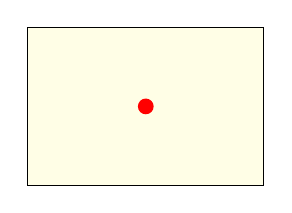
\begin{tikzpicture}
  \useasboundingbox (0,0) rectangle (3,2);
  \path[draw,fill=yellow!10] (0,0) rectangle (3,2);
  \path[fill=red] (1.5,1) circle [radius=1mm];
  \end{tikzpicture}
  }{
  The default method determines the map dimensions from a reference
  position and given document map dimensions.
  Also, a zoom level \refKey{mermap/supply/zoom}
  is required which relates to the Web Mercator map tile covering of the Earth.
  A higher zoom level gives a growing number of smaller map tiles.
  Alternative to the zoom level, a \meta{scale denominator} can be provided
  by \refKey{mermap/supply/flex area scale}, \refKey{mermap/flex scale}
  or \refKey{mermap/supply/flex reference scale} which determines
  the zoom level implicitly.
  As default, the reference position is the center of the map, but can be
  aligned at the map borders. This method is quite safe to use and could
  be the preferred one for many applications like showing the neighborhood
  of a route target.
  Finding the best reference point for depicting a certain area could
  be more tricky.
  }

\item \refKey{mermap/supply/type}|=|\docValue{areafit}:
  \tcbsidebyside[sidebyside adapt=left,blankest,grow to left by=1cm]
  {
  \tikzexternaldisable
  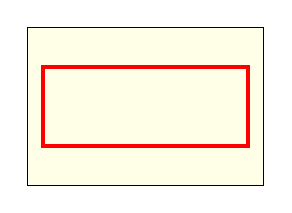
\begin{tikzpicture}
  \useasboundingbox (0,0) rectangle (3,2);
  \path[draw,fill=yellow!10] (0,0) rectangle (3,2);
  \path[draw=red,line width=0.5mm] (0.2,0.5) rectangle (2.8,1.5);
  \end{tikzpicture}
  }
  {
  The map dimensions are determined by an area with
  latitude and longitude boundaries which is fitted into given
  document map dimensions. The zoom level is computed accordingly
  for a fixed document tile size or by \refKey{mermap/supply/flex area fit}.
  In any case, the map contains the target area plus some protrusion.
  This method is also quite safe to use and may be
  the preferred one for many applications like showing a map which contains
  a bunch of markers (e.g. for locations of universities).
  If the map borders are required to exactly meet the boundaries,
  the third method can be regarded.
  }

\item \refKey{mermap/supply/type}|=|\docValue{boundaries}:
  \tcbsidebyside[sidebyside adapt=left,blankest,grow to left by=1cm]
  {
  \tikzexternaldisable
  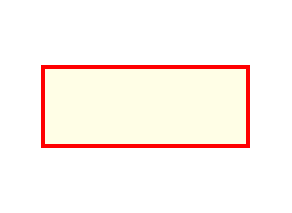
\begin{tikzpicture}
  \useasboundingbox (0,0) rectangle (3,2);
  \path[draw=red,line width=0.5mm,fill=yellow!10] (0.2,0.5) rectangle (2.8,1.5);
  \end{tikzpicture}
  }{
  The most obvious method determines the map dimensions from
  latitude and longitude boundaries. For this, a corresponding zoom level
  \refKey{mermap/supply/zoom}
  is required which relates to the Web Mercator map tile covering of the Earth.
  Alternative to the zoom level, a \meta{scale denominator} can be provided
  by \refKey{mermap/supply/flex area scale}
  or \refKey{mermap/supply/flex reference scale} which determines
  the zoom level implicitly.
  Note that a too high zoom level imposes the risk of downloading an unwanted
  high quantity of map tiles resulting in a much too large document map.
  Therefore, this most obvious method is \emph{not recommended} for the
  beginner and may be explored after some experience.
  }
\end{enumerate}



\clearpage
%-------------------------------------------------------------------------------
\subsection{Map Supply}

\begin{docCommand}{mrcsupplymap}{\oarg{options}\marg{definition}}
  The \meta{options} provide parameters for the Python~3 script to supply all
  materials for a map.
  All options share the common prefix |mermap/supply/|.\par
  The map is identified by\\
  \meta{id}=\refKey{mermap/definition prefix}+\meta{definition}\\
  for later drawing.
  This identifier \meta{id} has to be unique for the document.
  It corresponds to generated files \meta{id}|.def|, \meta{id}|.md5|, and
  possibly \meta{id}|.png|.
  Do not use spaces or special characters like umlauts for \meta{definition}.
  \par
  If \refCom{mrcactivatescript} is used inside the preamble,
  \refCom{mrcsupplymap} executes the Python~3 script, otherwise nothing happens.
\end{docCommand}


\begin{docCommand}{mermapsetsupply}{\marg{options}}
  Sets \meta{options} for all following maps inside the current \TeX\ group.
  All options share the common prefix |mermap/supply/|, e.g. for setting
  \refKey{mermap/supply/type} use
  \begin{dispListing}
    \mermapsetsupply{type=reference}
  \end{dispListing}
  Also see \refCom{mermapset} and \refCom{mermapsetmarker}.
\end{docCommand}


\begin{docMrcKey}{definition prefix}{=\meta{definition prefix}}{no default, initially |maps/|}
  Prefix for map identifiers and generated map files, see \refCom{mrcsupplymap}
  and \refCom{mrcapplymap}.
  Note that \refKey{mermap/definition prefix} is not to be used inside
  the option list for \refCom{mrcsupplymap}.
\end{docMrcKey}

\begin{docMrcKey}[supply]{type}{=\meta{type}}{no default, initially |reference|}
  The \meta{type} defines the basic computation for the map. Feasible values are
  \begin{itemize}
  \item\docValue{reference}: \flqq map with reference position\frqq\\
    The map is constructed from a given reference position
    \refKey{mermap/supply/latitude},\\
    \refKey{mermap/supply/longitude},\\
    a zoom level \refKey{mermap/supply/zoom},\\
    map dimensions\\
    \refKey{mermap/supply/width},\\
    \refKey{mermap/supply/height},\\
    and alignment \refKey{mermap/supply/align}.
  \item\docValue{areafit}: \flqq map fitting an area\frqq\\
    The map is constructed from a given area boundaries\\
    \refKey{mermap/supply/west},\\
    \refKey{mermap/supply/east},\\
    \refKey{mermap/supply/north},\\
    \refKey{mermap/supply/south},\\
    map dimensions\\
    \refKey{mermap/supply/width},\\
    \refKey{mermap/supply/height},\\
    and alignment \refKey{mermap/supply/align}.
  \item\docValue{boundaries}: \flqq map with boundaries\frqq\\
    The map is constructed from given boundaries\\
    \refKey{mermap/supply/west},\\
    \refKey{mermap/supply/east},\\
    \refKey{mermap/supply/north},\\
    \refKey{mermap/supply/south},\\
    and zoom level \refKey{mermap/supply/zoom}.
  \end{itemize}
\end{docMrcKey}

\pagebreak

\begin{docMrcKey}[supply]{zoom}{=\meta{setup zoom}}{no default, initially |9|}
  Map tile zoom factor alias $z$ coordinate of the map tiles.
  Used for map types \docValue{boundaries} and \docValue{reference}.
\end{docMrcKey}

\begin{docMrcKey}[supply]{north}{=\meta{setup north latitude}}{no default, initially |50|}
  Northern latitude degree, possibly negative for the southern hemisphere,
  lower than $90$ but always larger than \refKey{mermap/supply/south}.
  Used for map types \docValue{boundaries} and \docValue{areafit}.
\end{docMrcKey}

\begin{docMrcKey}[supply]{south}{=\meta{setup south latitude}}{no default, initially |48|}
  Southern latitude degree, possibly negative for the southern hemisphere,
  larger than $-90$ but always lower than \refKey{mermap/supply/north}.
  Used for map types \docValue{boundaries} and \docValue{areafit}.
\end{docMrcKey}

\begin{docMrcKey}[supply]{west}{=\meta{setup west longitude}}{no default, initially |11|}
  Western longitude degree, possibly negative for the western hemisphere,
  possibly shifted periodically, but always lower than \refKey{mermap/supply/east}.
  Used for map types \docValue{boundaries} and \docValue{areafit}.
\end{docMrcKey}

\begin{docMrcKey}[supply]{east}{=\meta{setup east longitude}}{no default, initially |13|}
  Eastern longitude degree, possibly negative for the western hemisphere,
  possibly shifted periodically, but always larger than \refKey{mermap/supply/west}.
  Used for map types \docValue{boundaries} and \docValue{areafit}.
\end{docMrcKey}


\begin{docMrcKeys}[
  doc keypath     = supply,
  doc parameter   = {=\marg{comma separated list of named positions}},
  doc description = {no default},
  %doc new         = 2020-05-04,
]{
  { doc name = area },
  { doc name = add area },
}
  Sets
  \refKey{mermap/supply/north}, \refKey{mermap/supply/south},
  \refKey{mermap/supply/west}, \refKey{mermap/supply/east}
  according to the given \meta{comma separated list of named positions}, i.e.
  the described area contains all these positions.\\
  \refKey{mermap/supply/area} resets the current area which requires
  at least two points inside the list.\\
  \refKey{mermap/supply/add area} does not reset the current area,
  i.e. the positions are added to the
  current area which possibly grows to fit all positions.\\
  Also note to take special care, if the international dateline is on your
  resulting map, see \Fullref{sec:dateline}.
  Used for map types \docValue{boundaries} and \docValue{areafit}
  or in combination with \refKey{mermap/supply/area to reference} also
  for for map type \docValue{reference}.
\end{docMrcKeys}



\begin{docMrcKeys}[
  doc keypath     = supply,
  doc parameter   = {=\marg{file name}},
  doc description = {no default},
  doc new         = 2020-05-08,
]{
  { doc name = area from marker input },
  { doc name = add area from marker input },
}
  Sets
  \refKey{mermap/supply/north}, \refKey{mermap/supply/south},
  \refKey{mermap/supply/west}, \refKey{mermap/supply/east}
  according to the given \refCom{mrcmarker} positions contained in a
  file with the given \meta{file name}.\\
  \refKey{mermap/supply/area from marker input} resets the current area which requires
  at least two marker positions inside the file.\\
  \refKey{mermap/supply/add area from marker input} does not reset the current area,
  i.e. the positions are added to the
  current area which possibly grows to fit all positions.\\
  Also note to take special care, if the international dateline is on your
  resulting map, see \Fullref{sec:dateline}.
  Used for map types \docValue{boundaries} and \docValue{areafit}
  or in combination with \refKey{mermap/supply/area to reference} also
  for for map type \docValue{reference}.
\end{docMrcKeys}



\begin{docMrcKey}[supply]{area to reference}{}{no value, initially unset}
  The map settings
  \refKey{mermap/supply/north}, \refKey{mermap/supply/south},
  \refKey{mermap/supply/west}, \refKey{mermap/supply/east}
  are taken to compute the map center. This center position is saved
  to \refKey{mermap/supply/latitude} and \refKey{mermap/supply/longitude}.
  Used for map type \docValue{reference}.
\end{docMrcKey}


\clearpage

\begin{docMrcKey}[supply]{latitude}{=\meta{setup latitude}}{no default, initially |49|}
  Latitude degree of a reference point, possibly negative for the southern hemisphere.
  Used for map type \docValue{reference}.
\end{docMrcKey}

\begin{docMrcKey}[supply]{longitude}{=\meta{setup longitude}}{no default, initially |12|}
  Longitude degree of a reference point, possibly negative for the western hemisphere.
  Used for map type \docValue{reference}.
\end{docMrcKey}


\begin{docMrcKey}[supply]{position}{=\meta{setup latitude}:\meta{setup longitude}}{no default, initially |49:12|}
  Latitude degree and longitude of a reference point.
  Used for map type \docValue{reference}.
\end{docMrcKey}


\begin{docMrcKey}[supply]{named position}{=\meta{name}}{style, no default}
  The \emph{named position} given by \meta{name} describes
  a reference point, see \Fullref{sec:names_positions}.
  Used for map type \docValue{reference}.
\end{docMrcKey}



\begin{docMrcKey}[supply]{width}{=\meta{setup width in tiles}}{no default, initially |4|}
  Width of the map as multiplicity of map tiles.
  Used for map types \docValue{reference} and \docValue{areafit}.
\end{docMrcKey}

\begin{docMrcKey}[supply]{tex width}{=\meta{width}}{style, no default}
  Width of the map as \TeX\ dimension.
  This is a style to compute \refKey{mermap/supply/width} according to
  the current \refKey{mermap/tile size}.
\end{docMrcKey}

\begin{docMrcKey}[supply]{height}{=\meta{setup height in tiles}}{no default, initially |4|}
  Height of the map as multiplicity of map tiles.
  Used for map types \docValue{reference} and \docValue{areafit}.
\end{docMrcKey}

\begin{docMrcKey}[supply]{tex height}{=\meta{width}}{style, no default}
  Height of the map as \TeX\ dimension.
  This is a style to compute \refKey{mermap/supply/height} according to
  the current \refKey{mermap/tile size}.
\end{docMrcKey}

\begin{docMrcKey}[supply]{align}{=\meta{setup alignment}}{no default, initially |center|}
  Alignment of reference point or area for map types \docValue{reference} and \docValue{areafit}.
  Feasible values are
  \docValue{northwest}, \docValue{north}, \docValue{northeast}, \docValue{west},
  \docValue{center}, \docValue{east}, \docValue{southwest},\docValue{south}, \docValue{southeast}.
\end{docMrcKey}

\begin{docMrcKey}[supply]{target}{=\meta{setup target}}{no default, initially |tiles|}
  Defines the type of output for the Python~3 script. Feasible values are:
  \begin{itemize}
  \item\docValue{none}: No tiles are downloaded and no merged map is generated, just map computation.
    This is the fastest method and needs no tile supplier.
  \item\docValue{tiles}: Download map tiles from a tile map service (TMS) \refKey{mermap/supply/url}.
    Compilation of a document with map tile takes longer than compilation
    with a merged map and transparency should not be used with tiles,
    but the resulting document is smaller than a document with merged maps.
  \item\docValue{mergedmap}: Download map tiles from a tile map service (TMS)
    \refKey{mermap/supply/url} and merge them into a single map picture.
    This speeds compilation and allows transparency effects, but
    the resulting document is possibly larger than a document with map tiles,
    because map tiles often are optimized 8-bit image files while the merged
    image is a 24-bit PNG file. Additionally, synergy effects of using the same map tiles
    for different maps are lost.
    Also, since the pixel map is clipped to full pixels, the resulting map
    may differ (shift/size) from the more accurate tile representation by
    one pixel.
  \item\docValue{wmsmap}: Download a single map from a web map service (WMS)
    \refKey{mermap/supply/url}. Internally, the package treats a WMS like
    a tile map service including all tile calculations. Actually, a single
    file is downloaded.
  \end{itemize}
\end{docMrcKey}

\enlargethispage*{1cm}

\begin{docMrcKey}[][doc new=2020-08-06]{fail on missing resource}{\colOpt{=true\textbar false}}{default |true|, initially |true|}
  If set to |true|, compilation stops with an error, if
  \refKey{mermap/supply/target} and \refKey{mermap/mapdef/resource} are different.
  Typically, this means that something went wrong while trying to download
  map tiles. Set this option temporarily to |false|,
  if the map tile service or the internet
  connection is expected to be unavailable only temporarily.
\end{docMrcKey}



\clearpage
\begin{docMrcKey}[supply]{url}{=\meta{setup URL}}{no default, initially empty}
  Here, the url format with placeholder |{z}{x}{y}| for map tile download is defined.
  \textbf{Be sure that you have the permission to download, save, and use
  the map tiles from that URL. Illegal downloads are not endorsed in any
  way.}
  \begin{dispListing}
    url={https://abc.efg.hij/{z}/{x}/{y}.png?apikey=12345678},
  \end{dispListing}
  See \Fullref{sec:maptileserver} for predefined URLs.
\end{docMrcKey}


\begin{docMrcKey}[supply]{url with api key}{=\marg{prefix}\marg{name}\marg{postfix}}{no default}
  This is an alternative version of \refKey{mermap/supply/url}.
  The URL is constructed from some fixed \meta{prefix} and \meta{postfix} with
  an API key in between. The API key is retrieved by \meta{name} from a
  repository filled by \refCom{mrcsetapikey}.
  \begin{dispListing}
    url={https://abc.efg.hij/{z}/{x}/{y}.png?apikey=}{myservice}{},
  \end{dispListing}
  See \Fullref{sec:maptileserver} for predefined URLs.
\end{docMrcKey}


\begin{docCommand}{mrcsetapikey}{\marg{name}\marg{value}}
  Stores an API key \meta{value} for access with the given \meta{name}.
  Typically, \meta{value} is a received ID from a map tile service provider
  after personal registration. \meta{name} is a placeholder which is used
  inside \refKey{mermap/supply/url with api key} to mark the insertion
  point for the API key.
  \begin{dispListing}
    \mrcsetapikey{myservice}{....K942XY....}
  \end{dispListing}
\end{docCommand}



\begin{docMrcKey}[supply]{attribution}{=\meta{attribution text}}{no default, initially empty}
  Attribution text for the map source. Typically, it acknowledges the copyright
  of the map data provider. It may contain hyperlinks.
  It is used to set up \refKey{mermap/mapdef/attribution} afterwards
  and it is accessible as \docAuxCommand{mrcmapattribution} (use read-only).\par
  For technical reasons, do not use \verb+"+. \docAuxCommand{mrcumlaut}
  may be used for masking umlauts, e.g. use \verb+\mrcumlaut{u}+ instead of
  \verb+\"{u}+, but umlauts can also be used directly, e.g. as UTF-8 coded characters.
\end{docMrcKey}

\begin{docMrcKey}[supply]{attribution print}{=\meta{attribution text}}{no default, initially empty}
  Attribution text for the map source.
  In contrast to \refKey{mermap/supply/attribution} it is intended for media
  that does not support hyperlinks like printed posters, books, etc.
  It is used to set up \refKey{mermap/mapdef/attribution print} afterwards
  and it is accessible as \docAuxCommand{mrcmapattributionprint} (use read-only).
\end{docMrcKey}


\begin{docMrcKey}[supply]{basename}{=\meta{setup tile base name}}{no default, initially \texttt{tiles/tile}}
  Prefix for local tile files, e.g. '|tiles/map|' for '|tiles/map_10_10_10.png|'.
\end{docMrcKey}


\clearpage
\begin{docMrcKey}[supply]{flex reference scale}{=\meta{scale denominator}}{no default}
  With the given \meta{scale denominator}, an appropriate \refKey{mermap/supply/zoom}
  and \refKey{mermap/tile size} is computed. Note that
  the \meta{scale denominator}
  always applies to the current \refKey{mermap/supply/latitude}
  and is used for map type \docValue{boundaries} and \docValue{reference}.
  For example, if the reference point is on the north side of the map,
  also the \meta{scale denominator}
  applies to the most northern latitude.

  Note to take special care to the order of the options.
  \begin{itemize}
  \item The reference point has to be set \emph{before}
    \refKey{mermap/supply/flex reference scale}, e.g. by
    \refKey{mermap/supply/latitude}, \refKey{mermap/supply/position},
    \refKey{mermap/supply/named position}.
  \item \refKey{mermap/supply/tex height}, \refKey{mermap/supply/tex width}
    (only for map type \docValue{reference})
    have to be set \emph{after} \refKey{mermap/supply/flex reference scale},
    because the \refKey{mermap/tile size} is adapted.
  \end{itemize}
  Also see \refKey{mermap/flex tile size}, \refKey{mermap/flex zoom},
  and \refKey{mermap/flex scale}.
\tikzsetnextfilename{maptiles_flex_reference_scale}%
\begin{dispExample}
\begin{tikzpicture}
  \mrcmap[type=reference,latitude=48.14,longitude=11.57,
    flex reference scale=250000,
    source=opentopomap,
    tex width=\linewidth,tex height=5cm]{}
  \mrcdrawmap
  \node[below,font=\fontsize{7pt}{7pt}\sffamily] at (mrcmap.south)
        {\mrcmapattribution};
  \mrcclipmap
  \path[draw] (mrcmap.south west) rectangle (mrcmap.north east);
  \node[below left=2mm,align=right,fill=white,fill opacity=0.5,
    text opacity=1] at (mrcmap.north east) {scale \mrcprettymapscale};
\end{tikzpicture}
\end{dispExample}
\end{docMrcKey}


\begin{docMrcKey}[supply]{flex area scale}{=\meta{scale denominator}}{no default}
  This is a shortcut for setting \refKey{mermap/supply/area to reference}
  and \refKey{mermap/supply/flex reference scale}=\meta{scale denominator}.
  Used for map type \docValue{boundaries} and \docValue{reference}.

  Note to take special care to the order of the options.
  \begin{itemize}
  \item The reference point has to be set \emph{before}
    \refKey{mermap/supply/flex area scale}.
  \item \refKey{mermap/supply/tex height}, \refKey{mermap/supply/tex width}
    (only for map type \docValue{reference})
    have to be set \emph{after} \refKey{mermap/supply/flex reference scale}.
  \end{itemize}
\end{docMrcKey}


\clearpage
\begin{docMrcKey}[supply]{flex area fit}{\colOpt{=\meta{size}}}{default |0pt|}
  This key can be used for map type \docValue{areafit} as \emph{final}
  option \emph{after} all other options.
  It applies a fine tuning to \refKey{mermap/tile size},
  \refKey{mermap/supply/width}, and \refKey{mermap/supply/height} such
  that the defined area fits exactly into the map region.
  If a \meta{size} is specified, width and height are reduced for the
  calculation by this \meta{size}, e.g. \meta{size}|=1cm| ensures a
  border of |5mm| on each side.
  Also see \refKey{mermap/flex tile size} and \refKey{mermap/flex zoom}.

\tikzsetnextfilename{maptiles_flex_area_fit}%
\begin{dispExample}
\begin{tikzpicture}
  \mrcNPdef{munich}{48.14}{11.58}
  \mrcNPdef{rio}{-22.91}{-43.20}
  \mrcNPdef{newyork}{40.71}{-74.01}
  \mrcmap[  type = areafit, area = {munich,rio,newyork},
    source=topplusopen web grau,
    tex width=\linewidth, tex height=7cm,
    flex area fit=1cm ]{}
  \mrcdrawmap
  \node[below,font=\fontsize{7pt}{7pt}\sffamily] at (mrcmap.south)
        {\mrcmapattribution};
  \draw[yellow] ([xshift=5mm,yshift=5mm]mrcmap.south west) rectangle
                ([xshift=-5mm,yshift=-5mm]mrcmap.north east);
  \draw[red,fill=red!50!gray!50!white,fill opacity=0.25]
    (\mrcNPcs{newyork}) -- (\mrcNPcs{rio}) -- (\mrcNPcs{munich}) -- cycle;
\end{tikzpicture}
\end{dispExample}
\end{docMrcKey}




\clearpage
\begin{docMrcKey}[supply]{pixel}{=\meta{setup pixel size}}{no default, initially |256|}
  Pixel width (and height) of a tile. It is especially needed for
  target \docValue{mergedmap} and also \docValue{wmsmap}.
  For \docValue{wmsmap}, it is multiplied with a pseudo tile calculation
  to compute the actual picture size to download.
\end{docMrcKey}


\begin{docMrcKey}[supply]{dpi}{=\meta{dpi value}}{style, no default}
  This style sets \refKey{mermap/supply/pixel} such that the given \meta{dpi value}
  is resulting (approximately).
  \begin{itemize}
  \item Note that this only applies for WMS Servers and not for
    TMS (Tile Map Service) Servers,
    because there \refKey{mermap/supply/pixel} is a fixed number depending on
    Server settings and cannot be chosen arbitrarily.
  \item A high \meta{dpi value} results in large downloaded map files.
    If the server does not provide a high resolution map, you will get
    unnecessary large files with blurred content.
  \item The \meta{dpi value} for TMS data can be changed by adapting
    \refKey{mermap/tile size} or \refKey{mermap/flex tile size}.
  \end{itemize}

\tikzsetnextfilename{maptiles_dpi_value}
\begin{dispExample}
\begin{tikzpicture}
 \mrcmap[type=reference,latitude=48.14,longitude=11.57,
    flex reference scale=250000,
    source=topplusopen p250, target=wmsmap, dpi=300,
    tex width=\linewidth,tex height=5cm]{dpi_value}
  \mrcdrawmap
  \node[below,font=\fontsize{7pt}{7pt}\sffamily] at (mrcmap.south)
        {\mrcmapattribution};
  \mrcclipmap
  \path[draw] (mrcmap.south west) rectangle (mrcmap.north east);
\end{tikzpicture}
\end{dispExample}

\end{docMrcKey}





%-------------------------------------------------------------------------------
\subsection{Map Apply}

\begin{docCommand}{mrcapplymap}{\marg{definition}}
  A map which is supplied by \refCom{mrcsupplymap} is applied
  inside a |tikzpicture| environment by
  \refCom{mrcapplymap} where \meta{definition} identifies the map.
  \refCom{mrcapplymap} replaces a manual setup by \refCom{mrcdefinemap}.
  The same map can be applied more than once inside a document.
  Note that applying a map does not mean to draw the map, but to prepare
  everything for drawing.
\end{docCommand}


\begin{docCommand}{mrcmap}{\oarg{options}\marg{definition}}
  This is a combination of
  \refCom{mrcsupplymap} with the given \meta{options}
  followed immediately by \refCom{mrcapplymap}.
  If \meta{definition} is left empty, an automated unique identifier is
  inserted.
  If a map is to be used just once, \refCom{mrcmap} may be preferred.
\end{docCommand}





\clearpage
%-------------------------------------------------------------------------------
\subsection{Map Tile Server}\label{sec:maptileserver}


To use map tiles with this package you obviously need access to a map tile server.
Thanks to all the many contributors to
\href{https://openstreetmap.org/copyright}{OpenStreetMap},
map data is free for everyone to use.
\textbf{But, map tile servers based on OpenStreetMap are not necessarily free}.

A list of online raster tile servers based on OpenStreetMap data is found here:\\
\url{https://wiki.openstreetmap.org/wiki/Raster_tile_providers}

\begin{itemize}
\item\bfseries I do not run a map tile server.
\item I do not and cannot grant any permission to access a map tile server.
\item I do not and cannot grant any permission to use map tiles in
  private, academic, free, or commercial publications.
\item All operators of map tile servers require to mention an attribution
  for their maps.
\end{itemize}

The following option allows easy usage of very few selected tile servers.
The tile server of \href{https://openstreetmap.org/copyright}{OpenStreetMap}
is not included because of its
\href{https://operations.osmfoundation.org/policies/tiles/}{Tile Usage Policy}.
I am aware that the following list could be enlarged much more, but I do not
want to add more to avoid any legal uncertainties.

\begin{itemize}
\item\bfseries I will remove an entry immediately, if the tile server operator
  asks for it.
\item\mdseries If \textbf{YOU} operate a tile server and you want an entry here, I would be
  glad to add it to the following list.
\end{itemize}

\medskip
\begin{docMrcKey}[supply]{source}{=\meta{source}}{style, no default}
  This style sets \refKey{mermap/supply/url}, \refKey{mermap/supply/attribution},\\
  \refKey{mermap/supply/attribution print} and \refKey{mermap/supply/basename}.\\
  Feasible values for \meta{source} are:
  %\mermapset{tile size=3.2512cm}
  \newcommand{\mapexample}[3][]{%
    \begingroup
    \mermapset{supply/source=#2}%
    \begin{itemize}
    \item Required attribution (\docAuxCommand{mrcmapattribution}):
      \begin{tcolorbox}[sharp corners,size=fbox,colback=yellow!8,colframe=yellow!80!gray,halign=flush left,before skip=2pt]
        \mrcmapattribution\end{tcolorbox}
    \item Required attribution for media without hyperlinks (\docAuxCommand{mrcmapattributionprint}):
      \begin{tcolorbox}[sharp corners,size=fbox,colback=yellow!8,colframe=yellow!80!gray,halign=flush left,before skip=2pt]
        \mrcmapattributionprint\end{tcolorbox}
    %\par\smallskip\
    \end{itemize}
    \endgroup\par\smallskip\tikzsetnextfilename{maptiles_#3}%
    \begin{tikzpicture}
    \mrcmap[source=#2,
      type=reference,latitude=48.14,longitude=11.58,zoom=7,
      tex width=\linewidth,tex height=2cm,#1]{#3}
      \mrcdrawmap
      \node[below,font=\fontsize{7pt}{7pt}\sffamily] at (mrcmap.south)
        {\mrcmapattribution};
    \end{tikzpicture}\par%
  }%
  \begin{itemize}

  \item\docValue{dummy}:\\
    Dummy tile server at loopback |127.0.0.1| for test purposes.

  \item\docValue{opentopomap}:\\
    Tile server (TMS) of \href{https://opentopomap.org/}{OpenTopoMap}.
    \begin{itemize}
    \item Usage (German language): \url{https://opentopomap.org/about#verwendung}
    \end{itemize}
    \mapexample{opentopomap}{opentopomap}

\clearpage
  \item\docValue{thunderforest opencyclemap}:\\
    Tile server of \href{https://www.thunderforest.com}{Thunderforest}.\\
    A registered \meta{api-key} is needed (free plan available)
    which is applied by\\
    \refCom{mrcsetapikey}\brackets{\docValue{thunderforest}}\marg{api-key}.
    \begin{itemize}
    \item Usage: \url{https://www.thunderforest.com/terms}
    \item API documentation: \url{https://www.thunderforest.com/maps/opencyclemap}
    \end{itemize}
    \mapexample{thunderforest opencyclemap}{thunderforest_opencyclemap}

  \item\docValue{thunderforest transport}:\\
    Tile server of \href{https://www.thunderforest.com}{Thunderforest}.\\
    A registered \meta{api-key} is needed (free plan available)
    which is applied by\\
    \refCom{mrcsetapikey}\brackets{\docValue{thunderforest}}\marg{api-key}.
    \begin{itemize}
    \item Usage: \url{https://www.thunderforest.com/terms}
    \item API documentation: \url{https://www.thunderforest.com/maps/transport}
    \end{itemize}
    \mapexample{thunderforest transport}{thunderforest_transport}

  \item\docValue{thunderforest landscape}:\\
    Tile server of \href{https://www.thunderforest.com}{Thunderforest}.\\
    A registered \meta{api-key} is needed (free plan available)
    which is applied by\\
    \refCom{mrcsetapikey}\brackets{\docValue{thunderforest}}\marg{api-key}.
    \begin{itemize}
    \item Usage: \url{https://www.thunderforest.com/terms}
    \item API documentation: \url{https://www.thunderforest.com/maps/landscape}
    \end{itemize}
    \mapexample{thunderforest landscape}{thunderforest_landscape}

\clearpage
  \item\docValue{thunderforest outdoors}:\\
    Tile server of \href{https://www.thunderforest.com}{Thunderforest}.\\
    A registered \meta{api-key} is needed (free plan available)
    which is applied by\\
    \refCom{mrcsetapikey}\brackets{\docValue{thunderforest}}\marg{api-key}.
    \begin{itemize}
    \item Usage: \url{https://www.thunderforest.com/terms}
    \item API documentation: \url{https://www.thunderforest.com/maps/outdoors}
    \end{itemize}
    \mapexample{thunderforest outdoors}{thunderforest_outdoors}

  \item\docValue{thunderforest atlas}:\tcbdocmarginnote{\tcbdocnew{2024-07-29}}\\
    Tile server of \href{https://www.thunderforest.com}{Thunderforest}.\\
    A registered \meta{api-key} is needed (free plan available)
    which is applied by\\
    \refCom{mrcsetapikey}\brackets{\docValue{thunderforest}}\marg{api-key}.
    \begin{itemize}
    \item Usage: \url{https://www.thunderforest.com/terms}
    \item API documentation: \url{https://www.thunderforest.com/maps/atlas}
    \end{itemize}
    \mapexample{thunderforest atlas}{thunderforest_atlas}

  \item\docValue{thunderforest transport-dark}:\\
    Tile server of \href{https://www.thunderforest.com}{Thunderforest}.\\
    A registered \meta{api-key} is needed (free plan available)
    which is applied by\\
    \refCom{mrcsetapikey}\brackets{\docValue{thunderforest}}\marg{api-key}.
    \begin{itemize}
    \item Usage: \url{https://www.thunderforest.com/terms}
    \item API documentation: \url{https://www.thunderforest.com/maps/transport-dark}
    \end{itemize}
    \mapexample{thunderforest transport-dark}{thunderforest_transport-dark}

\clearpage
  \item\docValue{thunderforest spinal-map}:\\
    Tile server of \href{https://www.thunderforest.com}{Thunderforest}.\\
    A registered \meta{api-key} is needed (free plan available)
    which is applied by\\
    \refCom{mrcsetapikey}\brackets{\docValue{thunderforest}}\marg{api-key}.
    \begin{itemize}
    \item Usage: \url{https://www.thunderforest.com/terms}
    \item API documentation: \url{https://www.thunderforest.com/maps/spinal-map}
    \end{itemize}
    \mapexample{thunderforest spinal-map}{thunderforest_spinal-map}

  \item\docValue{thunderforest pioneer}:\\
    Tile server of \href{https://www.thunderforest.com}{Thunderforest}.\\
    A registered \meta{api-key} is needed (free plan available)
    which is applied by\\
    \refCom{mrcsetapikey}\brackets{\docValue{thunderforest}}\marg{api-key}.
    \begin{itemize}
    \item Usage: \url{https://www.thunderforest.com/terms}
    \item API documentation: \url{https://www.thunderforest.com/maps/pioneer}
    \end{itemize}
    \mapexample{thunderforest pioneer}{thunderforest_pioneer}

  \item\docValue{thunderforest mobile-atlas}:\\
    Tile server of \href{https://www.thunderforest.com}{Thunderforest}.\\
    A registered \meta{api-key} is needed (free plan available)
    which is applied by\\
    \refCom{mrcsetapikey}\brackets{\docValue{thunderforest}}\marg{api-key}.
    \begin{itemize}
    \item Usage: \url{https://www.thunderforest.com/terms}
    \item API documentation: \url{https://www.thunderforest.com/maps/mobile-atlas}
    \end{itemize}
    \mapexample{thunderforest mobile-atlas}{thunderforest_mobile-atlas}

\clearpage
  \item\docValue{thunderforest neighbourhood}:\\
    Tile server of \href{https://www.thunderforest.com}{Thunderforest}.\\
    A registered \meta{api-key} is needed (free plan available)
    which is applied by\\
    \refCom{mrcsetapikey}\brackets{\docValue{thunderforest}}\marg{api-key}.
    \begin{itemize}
    \item Usage: \url{https://www.thunderforest.com/terms}
    \item API documentation: \url{https://www.thunderforest.com/maps/neighbourhood}
    \end{itemize}
    \mapexample{thunderforest neighbourhood}{thunderforest_neighbourhood}

  \item\docValue{topplusopen web}:\\
    Tile server (TMS) of \href{https://www.bkg.bund.de}{Bundesamt f\"{u}r Kartographie und Geod\"{a}sie}.
    \begin{itemize}
    \item Covers world / Europe / Germany depending on zoom level
    \item Usage (German language): \url{https://gdz.bkg.bund.de/index.php/default/digitale-geodaten/topplusopen-produkte.html}
    \end{itemize}
    \mapexample{topplusopen web}{topplusopen_web}

  \item\docValue{topplusopen web grau}:\\
    Tile server (TMS) of \href{https://www.bkg.bund.de}{Bundesamt f\"{u}r Kartographie und Geod\"{a}sie}.
    \begin{itemize}
    \item Covers world / Europe / Germany depending on zoom level
    \item Usage (German language): \url{https://gdz.bkg.bund.de/index.php/default/digitale-geodaten/topplusopen-produkte.html}
    \end{itemize}
    \mapexample{topplusopen web grau}{topplusopen_web_grau}

\clearpage
  \item\docValue{topplusopen web light}:\tcbdocmarginnote{\tcbdocnew{2024-07-29}}\\
    Tile server (TMS) of \href{https://www.bkg.bund.de}{Bundesamt f\"{u}r Kartographie und Geod\"{a}sie}.
    \begin{itemize}
    \item Covers world / Europe / Germany depending on zoom level
    \item Usage (German language): \url{https://gdz.bkg.bund.de/index.php/default/digitale-geodaten/topplusopen-produkte.html}
    \end{itemize}
    \mapexample{topplusopen web light}{topplusopen_web_light}

  \item\docValue{topplusopen web light grau}\tcbdocmarginnote{\tcbdocnew{2024-07-29}}:\\
    Tile server (TMS) of \href{https://www.bkg.bund.de}{Bundesamt f\"{u}r Kartographie und Geod\"{a}sie}.
    \begin{itemize}
    \item Covers world / Europe / Germany depending on zoom level
    \item Usage (German language): \url{https://gdz.bkg.bund.de/index.php/default/digitale-geodaten/topplusopen-produkte.html}
    \end{itemize}
    \mapexample{topplusopen web light grau}{topplusopen_web_light_grau}

\end{itemize}


\vfill
\begin{tcolorbox}[spartan,colback=white]
The following sources are Web map server (WMS). Therefore,
\refKey{mermap/supply/target} can only be set to \docValue{wmsmap}
or \docValue{none}.
\end{tcolorbox}
\clearpage

\begingroup
\ExplSyntaxOn
\int_gzero:N \g_tmpa_int
\NewDocumentCommand \cleanstep {}
{
  \fp_compare:nNnT { \g_tmpa_int-trunc(\g_tmpa_int/3)*3 } = 0
    {
      \int_compare:nNnT \g_tmpa_int > 0
        {
          \clearpage
        }
    }
  \int_gincr:N \g_tmpa_int
}
\ExplSyntaxOff

  \begin{itemize}

\foreach \name / \scdenom / \xtra in {p5/5000,p10/10000,p17.5/17500,p25/25000,p50/50000,p100/100000,p250/250000}
{
\cleanstep
  \item\docValue{topplusopen \name}:\\
    Web map server (WMS) of \href{https://www.bkg.bund.de}{Bundesamt f\"{u}r Kartographie und Geod\"{a}sie}.
    \begin{itemize}
    \item 1:\scdenom, covers Europe / Germany depending on zoom level
    \item Usage (German language): \url{https://gdz.bkg.bund.de/index.php/default/digitale-geodaten/topplusopen-produkte.html}
    \end{itemize}
    \mapexample[target=wmsmap]{topplusopen \name}{topplusopen_\name}

\cleanstep
  \item\docValue{topplusopen \name\ grau}:\\
    Web map server (WMS) of \href{https://www.bkg.bund.de}{Bundesamt f\"{u}r Kartographie und Geod\"{a}sie}.
    \begin{itemize}
    \item 1:\scdenom, covers Europe / Germany depending on zoom level
    \item Usage (German language): \url{https://gdz.bkg.bund.de/index.php/default/digitale-geodaten/topplusopen-produkte.html}
    \end{itemize}
    \def\grau{ grau}%
    \mapexample[target=wmsmap]{topplusopen \name\grau}{topplusopen_\name_grau}
}

  \end{itemize}
\endgroup

\end{docMrcKey}



\begin{docCommand}{mrcnewsupplysource}{\marg{source}\marg{options}}
  Adds a new \meta{source} value to \refKey{mermap/supply/source}.
  The \meta{options} should set the keys
  \refKey{mermap/supply/url}, \refKey{mermap/supply/attribution},\\
  \refKey{mermap/supply/attribution print} and \refKey{mermap/supply/basename}.
  It is recommend to use |x ...| for \meta{source} to avoid conflicts
  with future official additions to \refKey{mermap/supply/source}.
  \begin{dispListing}
  \mrcnewsupplysource{x example}
  {
    url               = https://127.0.0.1/dummy/{z}/{x}/{y}.png,
    attribution       = {Dummy tile server},
    attribution print = {Dummy tile server},
    basename          = tiles/dummy,
  }
  \end{dispListing}
\end{docCommand}



% !TeX root = mercatormap.tex
% !TeX encoding=UTF-8
% !TeX spellcheck=en_US
% include file of mercatormap.tex (manual of the LaTeX package mercatormap)
\clearpage
\section{Map Drawing}

%-------------------------------------------------------------------------------
\subsection{Principal Drawing}

\begin{docCommand}{mrcdrawmap}{\oarg{options}}
  Inside a |tikzpicture| environment, \refCom{mrcdrawmap} draws a map
  prepared by \refCom{mrcdefinemap}, \refCom{mrcapplymap}, or \refCom{mrcmap}.
  All \meta{options} share the common prefix |mermap/|.
  This is the principal macro to draw a prepared map respectively
  the background of the map. The background consists of downloaded map tiles
  or just a color rectangle.
\end{docCommand}

\begin{docMrcKey}{draw}{=\meta{tile draw}}{no default, initially |auto|}
  \begin{itemize}
  \item\docValue{auto}: Draws the map according to \refKey{mermap/mapdef/resource},
    i.e. downloaded maps or tiles are used, if available.
  \item\docValue{path}: Draws the map according to the style given by
    \refKey{mermap/map path}. Existing map tiles or merged maps are ignored
  \item\docValue{tiles}: Draws the map with downloaded map tiles, if
    available.
  \item\docValue{mergedmap}: Draws the map with a merged picture, if
    available.
  \item\docValue{wmsmap}: Draws the map with a downloaded WMS picture, if
    available.
  \end{itemize}
\end{docMrcKey}

\begin{docMrcKey}{map path}{=\meta{options}}{no default, initially |upper left=green!50,|\\|upper right=green!25, lower left=green!50!black!50, lower right=green!25|}
  Defines a \tikzname\ style for drawing the map without tiles.
  \meta{options} are feasible \tikzname\ path options.
\end{docMrcKey}

\begin{docMrcKey}{map clip}{=\meta{code}}{no default, initially \refCom{mrcclipmap}}
  Clipping options for the map. By default, the defined map is
  clipped with the full map rectangle. Use this option only, if you not want to clip
  the map to its specified size. \meta{code} is some \tikzname\ clipping code.
\end{docMrcKey}

\begin{docMrcKey}{map scope}{=\meta{options}}{no default, initially empty}
  \refCom{mrcdrawmap} uses a |scope| environment inside which takes
  the given \tikzname\ \meta{options}.
\end{docMrcKey}


\begin{docCommand}{mrcclipmap}{}
  Clips all subsequent drawings against the applied map.\\
  This is a shortcut macro identical to
  \begin{dispListing}
  \path[clip] (mrcmap.south west) rectangle (mrcmap.north east);
  \end{dispListing}
\end{docCommand}


\begin{docCommand}{mrcboundmap}{}
  Sets the picture bounding box according to the applied map.\\
  This is a shortcut macro identical to
  \begin{dispListing}
  \path[use as bounding box]
    (mrcmap.south west) rectangle (mrcmap.north east);
  \end{dispListing}
\end{docCommand}


\clearpage
%-------------------------------------------------------------------------------
\subsection{Flexible Tile Size}\label{sec:flexible_tile_size}

Typically, the pixel size of a map tile is fixed and a map tile is a
pixel graphics file. The actual size of such an included picture inside
the document is freely selectable. Note that a very small
\refKey{mermap/tile size} results in very small map lettering,
while a very large \refKey{mermap/tile size} results results in
very blurred images.

The general idea of a \emph{flexible} tile size is to specify an aspired
tile size called \refKey{mermap/flex tile size} and to give \LaTeX\
the freedom to select \refKey{mermap/tile size} in \emph{about the same size}
as \refKey{mermap/flex tile size}.
This freedom is used to achieve a \emph{pseudo zoom} called
\refKey{mermap/flex zoom} which is a nearly arbitrary rational number instead
of \refKey{mermap/supply/zoom} which is a natural number.

This \emph{pseudo zoom} is applied by several options which share \emph{flex}
in their names, e.g.
\refKey{mermap/flex scale}, \refKey{mermap/named flex scale},
\refKey{mermap/supply/flex reference scale},
\refKey{mermap/supply/flex area scale},
\refKey{mermap/supply/flex area fit}.



\begin{docMrcKey}{tile size}{=\meta{length}}{no default, initially |32.512mm|}
  Width and height of a drawn tile picture are set to \meta{length}.
  For standard tiles with 256 times 256 pixels a tile size of
  \SI{32.512}{mm} = \SI{1.28}{in} results in an approximate
  \SI{200}{dpi} output for the document.
  For a |beamer| document, consider to use a \refKey{mermap/tile size} of
  \SI{21.333333}{mm} to get approximate 1:1 pixel input and output (depending on |beamer| settings
  and used hardware). Also see \refKey{mermap/mapdef/tile size}.
\end{docMrcKey}

\begin{docMrcKey}{flex tile size}{=\meta{length}}{no default, initially |32.512mm|}
  Aspired width and height of a tile picture are set to \meta{length}.
  This value is used while applying \refKey{mermap/flex zoom}.
\end{docMrcKey}


\begin{docMrcKey}{flex zoom}{=\meta{pseudo zoom}}{style, no default}
  This style sets \refKey{mermap/supply/zoom} and \refKey{mermap/tile size} in combination.
  \begin{itemize}
  \item
    If \meta{pseudo zoom} is a natural number,
    \refKey{mermap/supply/zoom} is set to \meta{pseudo zoom} and
    \refKey{mermap/tile size} is set to \refKey{mermap/flex tile size}.
  \item Otherwise, \refKey{mermap/supply/zoom} is set to the natural number
    closest to \meta{pseudo zoom} and \refKey{mermap/tile size} is such
    enlarged or reduced that the \meta{pseudo zoom} value is simulated,
    i.e. the \emph{impression} of a rational zoom factor is given.
  \end{itemize}
  Note that \refKey{mermap/flex zoom} has to be used \emph{before}
  \refCom{mrcsupplymap} or \refCom{mrcmap}, because the zoom setup is
  adapted.
\end{docMrcKey}


\clearpage
\begin{docMrcKey}{flex scale}{=\meta{scale denominator}:\meta{latitude}}{style, no default}
  For different latitude scopes, an identical zoom factor produces maps of
  different scale. With \refKey{mermap/flex scale}, a \refKey{mermap/flex zoom}
  is computed to achieve the given \meta{scale denominator} at a given \meta{latitude}.
  Note that this only applies to the center of a map. If the produced
  map is not centered at \meta{latitude}, the produced scale may
  differ from the intended one.
  Also see \refKey{mermap/supply/flex reference scale}.

\tikzsetnextfilename{drawing_flex_scale}%
\begin{dispExample}
\begin{tikzpicture}
  \mermapset{flex scale=250000:48.14}
  \mrcmap[type=reference,latitude=48.14,longitude=11.57,
    source=opentopomap,
    tex width=\linewidth,tex height=5cm]{}
  \mrcdrawmap
  \node[below,font=\fontsize{7pt}{7pt}\sffamily] at (mrcmap.south)
        {\mrcmapattribution};
  \mrcclipmap
  \path[draw] (mrcmap.south west) rectangle (mrcmap.north east);
  \node[below left=2mm, align=right, fill=white, fill opacity=0.5,
      text opacity=1]
    at (mrcmap.north east) {scale \mrcprettymapscale};
\end{tikzpicture}
\end{dispExample}
\end{docMrcKey}



\begin{docMrcKey}{named flex scale}{=\meta{scale denominator}:\meta{name}}{style, no default}
  Identical to \refKey{mermap/flex scale}, but used the \emph{named position}
  \meta{name} to provide a \emph{latitude}, see \Fullref{sec:names_positions}.
  \begin{dispListing}
  \mrcNPdef{munich}{48.137222}{11.575556}
  \mermapset{named flex scale=250000:munich} % identical to the following
  \mermapset{flex scale=250000:\mrcNPlat{munich}}
  \end{dispListing}
\end{docMrcKey}



\clearpage
%-------------------------------------------------------------------------------
\subsection{Geodetic Network}

\begin{docCommand}{mrcdrawnetwork}{\oarg{options}}
  Draws a geodetic network with meridians and parallels.
  All \meta{options} share the common prefix |mermap/|.
  The displayed lines are selected automatically according to some tuning
  parameters.
  The map is sliced in \emph{about} maximal \refKey{mermap/network pieces} in each
  direction. Meridians and parallels share a minimal distance of
  \emph{about} \refKey{mermap/network distance}. The algorithm is
  allowed to violate these conditions \emph{somewhat}.

  Note that oversized maps are not supported, i.e. maps which are wider
  than \ang{360} in longitude. Here, meridians are expected to be missing
  or misplaced.

\tikzsetnextfilename{drawing_network}%
\begin{dispExample*}{center lower}
% \mrcsetapikey{thunderforest}{YOUR-API-KEY}  % registered key
\begin{tikzpicture}
  \mrcmap[  type = boundaries,
    west = -20, east = 40, south = 36, north = 65,
    source=thunderforest landscape,
    flex area scale=40 000 000 ]{}
  \mrcdrawmap
  \node[below,font=\fontsize{7pt}{7pt}\sffamily] at (mrcmap.south)
        {\mrcmapattribution};
  \mrcclipmap
  \mrcdrawnetwork
  \path[draw] (mrcmap.south west) rectangle (mrcmap.north east);
\end{tikzpicture}
\end{dispExample*}
\end{docCommand}


\begin{docMrcKey}{network pieces}{=\meta{number}}{no default, initially |8|}
  The map is sliced in \emph{about} maximal \meta{number} pieces in each
  direction. \meta{number} may be exceeded \emph{somewhat}.
  It is underrun to comply with \refKey{mermap/network distance}.
\end{docMrcKey}


\begin{docMrcKey}{network distance}{=\meta{mesh width}}{no default, initially |2cm|}
  Meridians and parallels share a minimal distance of
  \emph{about} \meta{mesh width}.
  \meta{mesh width} may be underrun \emph{somewhat}.
  It is exceeded to comply with \refKey{mermap/network pieces}.
  For parallels on small scale maps, it refers to an averaged mesh width.
\end{docMrcKey}

\begin{docMrcKey}{network font}{=\meta{text}}{no default, initially
  |\textbackslash fontsize\brackets{4pt}\brackets{4pt}\textbackslash sffamily|}
  \meta{text} is some font setting for the latitude and longitude display.
\end{docMrcKey}



\subsection{Graphical Debug Overlay}

\begin{docCommand}{mrcdrawinfo}{}
  Draws some map information overlay for debugging purposes only.
  \tikzsetnextfilename{drawing_mrcdrawinfo}%
  \begin{dispExample}
  \begin{tikzpicture}
    \mrcNPdef{munich}{48.137222}{11.575556}
    \mrcmap[type=reference, named position=munich, source=opentopomap,
      flex reference scale=50000,
      tex width=\linewidth,tex height=10cm]{}
    \mrcdrawmap
    \node[below,font=\fontsize{7pt}{7pt}\sffamily] at (mrcmap.south)
          {\mrcmapattribution};
    \mrcclipmap
    \mrcdrawinfo
  \end{tikzpicture}
  \end{dispExample}
\end{docCommand}

% !TeX root = mercatormap.tex
% !TeX encoding=UTF-8
% !TeX spellcheck=en_US
% include file of mercatormap.tex (manual of the LaTeX package mercatormap)
\clearpage
\section{Scales and Sizes}%

Inside a defined map several size values and scaling options are
available. Please note that due to the nature of the Mercator projection and several
simplifying assumptions all specifications for map scale, map width, map height,
etc. are imprecise in the best case and even misleading in the worst case.
They are suited for representative diagrams,
but not for critical navigation purposes etc.

\subsection{Map Sizes and Document Sizes}

\begin{docCommand}{mrctexwidth}{}
  \TeX\ length denoting the document width of the current map.
\end{docCommand}

\begin{docCommand}{mrctexheight}{}
  \TeX\ length denoting the document width of the current map.
\end{docCommand}

\begin{docCommand}{mrcscale}{}
  Scaling factor between map and real world.
  A \TeX\ length given in |pt|, but stripped from that unit,
  multiplied by \refCom{mrcscale} corresponds to a real world length
  given in kilometers.
  Note that this is \emph{not} the map scale.
  Actually, it is reciprocal proportional to the map scale
  and proportional to the map scale denominator, see \refCom{mrcmapscaledenominator}.
\end{docCommand}

\begin{docCommand}{mrctextokm}{\marg{length}}
  Computes a given \TeX\ \meta{length} (with unit) into the corresponding
  real world length in kilometers (without unit).
  \begin{dispListing}
  Map width: \mrctextokm{\mrctexwidth}\,km
  \end{dispListing}
\end{docCommand}

\begin{docCommand}{mrctextomile}{\marg{length}}
  Computes a given \TeX\ \meta{length} (with unit) into the corresponding
  real world length in miles (without unit).
  \begin{dispListing}
  Map width: \mrctextomile{\mrctexwidth}\,mi
  \end{dispListing}
\end{docCommand}

\begin{docCommand}{mrckmtotex}{\marg{number}}
  Computes real world length \meta{number} in kilometers (without unit)
  to a \TeX\ length (with unit).
  \begin{dispListing}
  % draw a circle with radius 20km
  \draw (mrcpos) circle (\mrckmtotex{20});
  \end{dispListing}
\end{docCommand}

\begin{docCommand}{mrcmiletotex}{\marg{number}}
  Computes real world length \meta{number} in miles (without unit)
  to a \TeX\ length (with unit).
  \begin{dispListing}
  % draw a circle with radius 20 miles
  \draw (mrcpos) circle (\mrcmiletotex{20});
  \end{dispListing}
\end{docCommand}

\begin{docCommand}{mrcmapscaledenominator}{}
  Approximate map scale denominator.
  \SI{1}{cm} on the map corresponds approximately to
  \mbox{\refCom{mrcmapscaledenominator}$\cdot$\SI{1}{cm}} in the real world.
  Do not confuse with \refCom{mrcscale}.
  \begin{dispListing}
  Map scale: 1:\mrcmapscaledenominator
  \end{dispListing}
\end{docCommand}


\subsection{Pretty Size Output}


\begin{docCommand}{mrcprettymapscale}{}
  Approximate map scale given with three valid digits
  with a representation like |1:1000|.
  \begin{dispListing}
  Map scale: \mrcprettymapscale
  \end{dispListing}
\end{docCommand}

\begin{docCommand}{mrcprettymapwidth}{}
  Approximate map width in kilometers (or meters) with three valid digits:
  \begin{dispListing}
  Map width: \mrcprettymapwidth
  \end{dispListing}
  To create a pretty printing to your own liking, you can do like the
  following:
  \begin{dispListing}
  \newcommand{\myprettymapwidth}{\SI[round-mode=figures,round-precision=3]%
    {\mrctextokm{\mrctexwidth}}{km}}
  \end{dispListing}
\end{docCommand}

\begin{docCommand}{mrcprettymapheight}{}
  Approximate map height in kilometers (or meters) with three valid digits:
  \begin{dispListing}
  Map height: \mrcprettymapheight
  \end{dispListing}
\end{docCommand}


\begin{docCommand}{mrcprettymapresolution}{}
  Approximate map resolution in dpi (dots per inch):
  \begin{dispListing}
  Map resolution: \mrcprettymapresolution
  \end{dispListing}
\end{docCommand}

\begin{docCommand}{mrcprettytilesize}{}
  Approximate tile size inside the document (\TeX\ size) in millimeters:
  \begin{dispListing}
  \TeX\ tile size: \mrcprettytilesize
  \end{dispListing}
\end{docCommand}


\tikzsetnextfilename{scales_example}%
\begin{dispExample}
\begin{tikzpicture}
  \mrcNPdef{rome}{41.89300}{12.48557}
  \mermapset{named flex scale=2000000:rome}
  \mrcmap[type=reference, named position=rome, source=topplusopen web,
    tex width=\linewidth, tex height=10cm]{scales_example}
  \mrcdrawmap
  \node[below,font=\fontsize{7pt}{7pt}\sffamily] at (mrcmap.south)
        {\mrcmapattribution};
  \mrcclipmap
  \path[draw] (\mrcNPcs{rome}) circle (\mrckmtotex{50});
  \node[above] at ([yshift=\mrckmtotex{50}]\mrcNPcs{rome}) {\SI{50}{km}};
  \node[above right,fill=white,fill opacity=0.5,text opacity=1,align=center,
    line width=0pt, inner sep=2mm]
    at (mrcmap.south west) { \begin{tabular}{rl}
      scale:           & \mrcprettymapscale\\
      map width:       & \mrcprettymapwidth\\
      map height:      & \mrcprettymapheight\\
      \TeX\ tile size: & \mrcprettytilesize\\
      resolution:      & \mrcprettymapresolution
      \end{tabular}\\
      \begin{tikzpicture}
      \mrcdrawscalebar[width-in-km=100]
      \path[every node/.style={above,inner sep=0.5mm,font=\sffamily\tiny}]
        (mrcscalebar.north west) -- (mrcscalebar.north east)
        node[pos=0]{0} node[pos=0.2]{20} node[pos=0.4]{40} node[pos=0.6]{60}
        node[pos=0.8]{80} node[pos=1]{100} node[pos=1,right,yshift=-1mm]{km};
      \end{tikzpicture}
    };
\end{tikzpicture}
\end{dispExample}


\clearpage
\subsection{Scale Bars}


\begin{docCommand}{mrcdrawscalebar}{\oarg{options}}
  Draws a scale bar according to the given \meta{options}.
  All \meta{options} share the common prefix |mermap/scalebar/|.
  The most essential option is the \emph{width} of the scale bar.

  \tikzsetnextfilename{scales_scalebar1}
  \begin{dispExample}
  \begin{tikzpicture}
    \mrcNPdef{munich}{48.137222}{11.575556}
    \mrcNPdef{vienna}{48.208333}{16.373056}
    \mrcmap[tex width=\linewidth, tex height=4cm, target=none,
      type=areafit, area={munich,vienna}, flex area fit=2cm]{}
    \mrcdrawmap
    \mrcmarker{named position=munich, contents={M\"unchen}}
    \mrcmarker{named position=vienna, contents={Wien}}
    \mrcdrawscalebar[width-in-km=100, solid,
      at={([xshift=-10mm,yshift=5mm]mrcmap.south east)},
      placement={above left},  ]
  \end{tikzpicture}
  \end{dispExample}

  The size, position, and appearance of the scale bar can be customized by
  setting the various \meta{options}. The shape of the scale bar
  is denoted by a \tikzname\ node \docNode{mrcscalebar} which can be used
  for lettering.

  \enlargethispage*{1cm}
  \tikzsetnextfilename{scales_scalebar2}
  \begin{dispExample}
  \begin{tikzpicture}
    \mrcNPdef{munich}{48.137222}{11.575556}
    \mrcNPdef{vienna}{48.208333}{16.373056}
    \mrcmap[tex width=\linewidth, tex height=4cm, target=none,
      type=areafit, area={munich,vienna}, flex area fit=2cm]{}
    \mrcdrawmap
    \mrcmarker{named position=munich, contents={M\"unchen}}
    \mrcmarker{named position=vienna, contents={Wien}}
    \mrcdrawscalebar[width-in-km=100,solid,south-west-inside=10mm;3mm ]
    \path[every node/.style={above,inner sep=0.5mm,font=\sffamily\tiny}]
      (mrcscalebar.north west) -- (mrcscalebar.north east)
      node[pos=0]{0} node[pos=0.2]{20} node[pos=0.4]{40} node[pos=0.6]{60}
      node[pos=0.8]{80} node[pos=1]{100} node[pos=1,right,yshift=-1mm]{km};
  \end{tikzpicture}
  \end{dispExample}
\end{docCommand}

\clearpage

\begin{docMrcKey}[scalebar]{width-in-km}{=\meta{number}}{no default, initially |0|}
  Sets the width of the scale bar to match the real word length \meta{number}
  in kilometers.
\end{docMrcKey}

\begin{docMrcKey}[scalebar]{width-in-kilometer}{=\meta{number}}{no default, initially |0|}
  Alias for \refKey{mermap/scalebar/width-in-km}
\end{docMrcKey}

\begin{docMrcKey}[scalebar]{width-in-meter}{=\meta{number}}{no default, initially |0|}
  Sets the width of the scale bar to match the real word length \meta{number}
  in meters.
\end{docMrcKey}

\begin{docMrcKey}[scalebar]{width-in-mile}{=\meta{number}}{no default, initially |0|}
  Sets the width of the scale bar to match the real word length \meta{number}
  in miles.
\end{docMrcKey}

\begin{docMrcKey}[scalebar]{width-in-yard}{=\meta{number}}{no default, initially |0|}
  Sets the width of the scale bar to match the real word length \meta{number}
  in yards.
\end{docMrcKey}

\begin{docMrcKey}[scalebar]{partitions}{=\meta{number}}{no default, initially |5|}
  Determines the \meta{number} of partitions for the scale bar. If \meta{number}
  is set to 1, there is no partitioning.
\end{docMrcKey}

\begin{docMrcKey}[scalebar]{height}{=\meta{length}}{no default, initially |2mm|}
  Sets the height of the scale bar to the given \TeX\ \meta{length}.
\end{docMrcKey}


\begin{docMrcKey}[scalebar]{at}{=\marg{\tikzname\ coordinate}}{no default,
    initially \texttt{\brackets{(0,0)}}}
  The scale bar is positioned at the given \meta{\tikzname\ coordinate}.
  The placement is done with the \refKey{mermap/scalebar/placement} option.
  Both option correspond to the \tikzname\ options for positioning nodes.
  The scale bar can be positioned outside the map (e.g. below), but
  remember to use \refCom{mrcclipmap} \emph{after} the scale bar
  in this case, if needed.

%  \begin{dispListing}
%  \mrcdrawscalebar[
%     at        = {([xshift=-10mm,yshift=5mm]mrcmap.south east)},
%     placement = above left,
%    ]
%  \end{dispListing}

  \tikzsetnextfilename{scales_scalebar3}
  \begin{dispExample}
  \begin{tikzpicture}
    \mrcNPdef{munich}{48.137222}{11.575556}
    \mrcNPdef{vienna}{48.208333}{16.373056}
    \mrcmap[tex width=\linewidth, tex height=4cm, target=none,
      type=areafit, area={munich,vienna}, flex area fit=2cm]{}
    \mrcdrawmap
    \mrcmarker{named position=munich, contents={M\"unchen}}
    \mrcmarker{named position=vienna, contents={Wien}}
    \mrcdrawscalebar[width-in-km=200, partitions=8,
      at={([xshift=5mm,yshift=-2mm]mrcmap.south west)},
      placement=below right   ]
    \path[every node/.style={below,inner sep=0.5mm,font=\sffamily\tiny}]
      (mrcscalebar.south west) -- (mrcscalebar.south east)
      node[pos=0]{0} node[pos=0.25]{50} node[pos=0.5]{100} node[pos=0.75]{150}
      node[pos=1]{200} node[pos=1,right,yshift=1mm]{km};
  \end{tikzpicture}
  \end{dispExample}
\end{docMrcKey}

\pagebreak

\begin{docMrcKey}[scalebar]{placement}{=\meta{\tikzname\ positioning}}{no default, initially empty}
  \meta{\tikzname\ positioning} of a scale bar in combination with
  \refKey{mermap/scalebar/at}. All \tikzname\ placement options for nodes
  can be used, e.g. \texttt{above left} or \texttt{anchor=mid west}, etc.
  Actually, \emph{any} node option could be applied here, but the intended use
  is for placement options only.
\end{docMrcKey}


\begin{docMrcKey}[scalebar]{south-east-inside}{\colOpt{=\meta{x shift};\meta{y shift}}}{default |0pt;0pt|, initially unset}
  Shortcut for placing the scale bar at the south east corner of the map.
  The optional \mbox{\meta{x shift}} and \meta{y shift} denote the
  absolute shift values in each direction, i.e. the algebraic sign is
  automatically complemented.
  If only \meta{x shift} is given, then \meta{y shift} is set
  to the same value. \refKey{mermap/scalebar/at} and \refKey{mermap/scalebar/placement}
  are set by this option.
\end{docMrcKey}

\begin{docMrcKey}[scalebar]{south-east-outside}{\colOpt{=\meta{x shift};\meta{y shift}}}{default |0pt;0pt|, initially unset}
  Shortcut for placing the scale bar below the south east corner of the map.
\end{docMrcKey}

\begin{docMrcKey}[scalebar]{south-west-inside}{\colOpt{=\meta{x shift};\meta{y shift}}}{default |0pt;0pt|, initially unset}
  Shortcut for placing the scale bar at the south west corner of the map.
\end{docMrcKey}

\begin{docMrcKey}[scalebar]{south-west-outside}{\colOpt{=\meta{x shift};\meta{y shift}}}{default |0pt;0pt|, initially unset}
  Shortcut for placing the scale bar below the south west corner of the map.
\end{docMrcKey}

\begin{docMrcKey}[scalebar]{north-west-inside}{\colOpt{=\meta{x shift};\meta{y shift}}}{default |0pt;0pt|, initially unset}
  Shortcut for placing the scale bar at the north west corner of the map.
\end{docMrcKey}

\begin{docMrcKey}[scalebar]{north-west-outside}{\colOpt{=\meta{x shift};\meta{y shift}}}{default |0pt;0pt|, initially unset}
  Shortcut for placing the scale bar above the north west corner of the map.
\end{docMrcKey}

\begin{docMrcKey}[scalebar]{north-east-inside}{\colOpt{=\meta{x shift};\meta{y shift}}}{default |0pt;0pt|, initially unset}
  Shortcut for placing the scale bar at the north east corner of the map.
\end{docMrcKey}

\begin{docMrcKey}[scalebar]{north-east-outside}{\colOpt{=\meta{x shift};\meta{y shift}}}{default |0pt;0pt|, initially unset}
  Shortcut for placing the scale bar above the north east corner of the map.
\end{docMrcKey}


\begin{docMrcKey}[scalebar]{major style}{=\marg{\tikzname\ options}}{no default, initially empty}
  The \emph{major} part of the scale bar is a single \tikzname\ path object
  which can be customized by the given \meta{\tikzname\ options}.
  The \emph{major} part consists of the black area in the default case.
  \tikzsetnextfilename{scales_scalebar4}
  \begin{dispExample}
  \begin{tikzpicture}
    \mrcdrawscalebar[scale=2000000, width-in-km=100,
        major style={left color=red,right color=blue}   ]
  \end{tikzpicture}
  \end{dispExample}
\end{docMrcKey}


\begin{docMrcKey}[scalebar]{minor style}{=\marg{\tikzname\ options}}{no default, initially empty}
  The \emph{minor} part of the scale bar is a single \tikzname\ path object
  which can be customized by the given \meta{\tikzname\ options}.
  The \emph{minor} part is seen as holes in the default case.
  \refKey{mermap/scalebar/minor style} has only an effect, if
  the minor part is drawn \refKey{mermap/scalebar/solid}.
  \tikzsetnextfilename{scales_scalebar5}
  \begin{dispExample}
  \begin{tikzpicture}
    \mrcdrawscalebar[scale=2000000, width-in-km=100, solid,
         minor style={yellow}  ]
  \end{tikzpicture}
  \end{dispExample}
\end{docMrcKey}


\pagebreak
\begin{docMrcKey}[scalebar]{double}{\colOpt{=true\textbar false}}{default |true|, initially |true|}
  If set to |true|, the scale bar is drawn as a double ruler.
\end{docMrcKey}


\begin{docMrcKey}[scalebar]{single}{\colOpt{=true\textbar false}}{default |true|, initially |false|}
  If set to |true|, the scale bar is drawn as a single ruler.
  \refKey{mermap/scalebar/single} is inverse to \refKey{mermap/scalebar/double}.
  \tikzsetnextfilename{scales_scalebar6}
  \begin{dispExample}
  \begin{tikzpicture}
    \mrcdrawscalebar[scale=2000000, width-in-km=100, single, height=1mm]
  \end{tikzpicture}
  \end{dispExample}
\end{docMrcKey}


\begin{docMrcKey}[scalebar]{transparent}{\colOpt{=true\textbar false}}{default |true|, initially |true|}
  If set to |true|, the \emph{minor} part of the scale bar is drawn transparent,
  i.e. as holes inside the ruler.
\end{docMrcKey}


\begin{docMrcKey}[scalebar]{solid}{\colOpt{=true\textbar false}}{default |true|, initially |false|}
  If set to |true|, the \emph{minor} part of the scale bar is drawn opaque.
  It is drawn white or according to \refKey{mermap/scalebar/minor style}.
  \refKey{mermap/scalebar/solid} is inverse to \refKey{mermap/scalebar/transparent}.
\end{docMrcKey}


\begin{docMrcKey}[scalebar]{scale}{=\meta{scale denominator}}{no default, initially unset}
  Sets or overwrites the \meta{scale denominator} setting.
  \textbf{Using this key is not needed and may even lead to erroneous displays
    inside a |tikzpicture| with a defined map setting.}
  This key is helpful, if a scale bar is used without a defined map.
\end{docMrcKey}


% !TeX root = mercatormap.tex
% !TeX encoding=UTF-8
% !TeX spellcheck=en_US
% include file of mercatormap.tex (manual of the LaTeX package mercatormap)
\clearpage
\section{Markers}%
As described before, a map can be amended by arbitrary \tikzname\ code
using map coordinates.
For highlighting places or adding markers, the \refCom{mrcmarker} macro
may be helpful which provides some predefined marker types.

%-------------------------------------------------------------------------------
\subsection{Marker Settings}

\begin{docCommand}{mrcmarker}{\marg{options}}
  Places a marker according to the given \meta{options} on the map.
  All \meta{options} share the common prefix |mermap/marker/|.
  Different \refKey{mermap/marker/type} settings are available which are
  more or less customizable.

\tikzsetnextfilename{marker_mrcmarker}%
\begin{dispExample}
% \mrcsetapikey{thunderforest}{YOUR-API-KEY} % registered key
\begin{tikzpicture}
  \mrcmap[type=reference, position=48.15:11.6,
    flex reference scale=500 000,
    source=thunderforest neighbourhood,
    tex width=\linewidth,tex height=4cm]{}
  \mrcdrawmap
  \node[below,font=\fontsize{7pt}{7pt}\sffamily] at (mrcmap.south)
    {\mrcmapattribution};
  \mrcdrawnetwork
  \mrcclipmap
  \mermapsetmarker{draw=red, fill=red!20!white, font=\sffamily\footnotesize}
  \mrcmarker{type=classic, position=48.15:11.2, contents={A}, radius=0.5mm}
  \mrcmarker{type=pin,     position=48.15:11.3, contents={B}}
  \mrcmarker{type=pinflip, position=48.15:11.4, contents={C}}
  \mrcmarker{type=drop,    position=48.15:11.5, contents={D}}
  \mrcmarker{type=knob,    position=48.15:11.6, contents={E}}
  \mrcmarker{type=pictodropring, position=48.15:11.7, contents={F}}
  \mrcmarker{type=pictoknobring, position=48.15:11.8, contents={G}}
  \mrcmarker{type=ringx,   position=48.15:11.9, contents={H}}
  \mrcmarker{type=markx,   position=48.15:12,   contents={I}}
\end{tikzpicture}
\end{dispExample}
\end{docCommand}


\begin{docCommand}{mermapsetmarker}{\marg{options}}
  Sets \meta{options} for all following markers inside the current \TeX\ group.
  All options share the common prefix |mermap/marker/|, e.g. for setting
  \refKey{mermap/marker/type} use
  \begin{dispListing}
    \mermapsetmarker{type=pin}
  \end{dispListing}
  Also see \refCom{mermapset} and \refCom{mermapsetsupply}.
\end{docCommand}

\pagebreak

\begin{docMrcKey}[marker]{first options}{=\meta{options}}{no default, initially unset}
  The given list of \meta{options} is used inside every \refCom{mrcmarker}
  \emph{before} the options of \refCom{mrcmarker}.
\end{docMrcKey}

\begin{docMrcKey}[marker]{last options}{=\meta{options}}{no default, initially unset}
  The given list of \meta{options} is used inside every \refCom{mrcmarker}
  \emph{after} the options of \refCom{mrcmarker}.
\end{docMrcKey}

\begin{docMrcKey}[marker]{latitude}{=\meta{latitude}}{no default, initially |12|}
  Latitude degree of the place marker.
  It is accessible as \docAuxCommand{mrcmarkerlatitude} (use read-only).
\end{docMrcKey}

\begin{docMrcKey}[marker]{lat}{=\meta{latitude}}{no default, initially |12|}
  Alias for \refKey{mermap/marker/latitude}.
\end{docMrcKey}

\begin{docMrcKey}[marker]{longitude}{=\meta{longitude}}{no default, initially |49|}
  Longitude degree of the place marker.
  It is accessible as \docAuxCommand{mrcmarkerlongitude} (use read-only).
\end{docMrcKey}

\begin{docMrcKey}[marker]{lon}{=\meta{longitude}}{no default, initially |49|}
  Alias for \refKey{mermap/marker/longitude}.
\end{docMrcKey}

\begin{docMrcKey}[marker]{position}{=\meta{place latitude}:\meta{place longitude}}{no default, initially |12:49|}
  Sets the latitude degree and the longitude degree of the place marker.
\end{docMrcKey}

\begin{docMrcKey}[marker]{named position}{=\meta{name}}{style, no default}
  Sets the latitude degree and the longitude degree of the place marker
  to the \emph{named position} denoted by \meta{name}, see \Fullref{sec:names_positions}.
\end{docMrcKey}

\begin{docMrcKey}[marker]{use inside}{=\meta{area}}{no default, initially |map|}
  The place marker is used or ignored according to its belonging inside the
  given \meta{area}. Feasible values for \meta{area} are:
  \begin{itemize}
  \item\docValue{map}: Use inside map.
  \item\docValue{vicinity}: Use inside map plus vicinity, see \refKey{mermap/vicinity}.
  \end{itemize}
\end{docMrcKey}


\begin{docMrcKey}[marker]{contents}{=\meta{text}}{no default, initially empty}
  Sets \meta{text} for displaying inside the marker, if
  the marker type supports such a thing.
  It is accessible as \docAuxCommand{mrcmarkercontents} (use read-only).
\end{docMrcKey}

\begin{docMrcKey}[marker]{pictocontents}{=\meta{code}}{no default, initially empty}
  Sets \tikzname\ \meta{code} for displaying inside the marker, if
  the marker type supports such a thing.
  It is accessible as \docAuxCommand{mrcmarkerpictocontents} (use read-only).
\end{docMrcKey}

\begin{docMrcKey}[marker]{alias}{=\meta{text}}{no default, initially |noname|}
  The position of the marker is available as \tikzname\ coordinate by
  the given \meta{text}, e.g. to draw to or from the marker.
\end{docMrcKey}

\begin{docMrcKey}[marker][doc updated=2020-05-04]{uuid}{=\meta{uuid}}{no default, initially empty}
  Sets a \meta{uuid} for unique identification of markers.
  It is accessible as \docAuxCommand{mrcmarkeruuid} (use read-only)
  and \docAuxCommand[doc sort index=mermap_marker_uuid_tl]{l_mermap_marker_uuid_tl} (use read-only).
  The \meta{uuid} is provided for user applications.
\end{docMrcKey}

\begin{docMrcKeys}[
  doc keypath     = marker,
  doc name        = generic,
  doc parameter   = {=\meta{text}},
  doc description = {no default, initially empty},
  doc new         = 2020-05-04,
]{}
  Sets \meta{text} as generic content for user applications.
  It is accessible as \docAuxCommand{mrcmarkergeneric} (use read-only)
  and \docAuxCommand[doc sort index=mermap_marker_generic_tl]{l_mermap_marker_generic_tl} (use read-only).
\end{docMrcKeys}


\begin{docMrcKey}[marker]{category}{=\meta{category}}{no default, initially empty}
  Sets a \meta{category} to group markers.
  It is accessible as \docAuxCommand{mrcmarkercategory} (use read-only).
\end{docMrcKey}

\clearpage

\begin{docMrcKey}[marker]{show}{\colOpt{=true\textbar false}}{default |true|, initially |true|}
  If set to |true|, the marker is shown, if it lies inside the map (or vicinity).
  Otherwise, the place marker is not used.
\end{docMrcKey}


\begin{docMrcKey}[marker]{hide}{\colOpt{=true\textbar false}}{default |true|, initially |false|}
  If set to |true|, the marker is not used.
  \refKey{mermap/marker/hide} is inverse to \refKey{mermap/marker/show}.
\end{docMrcKey}



\begin{docMrcKey}[marker]{show category}{=\meta{category}}{style, no default}
  Sets \refKey{mermap/marker/show} to |true|, if \refKey{mermap/marker/category} equals \meta{category}.
  Otherwise, nothing happens.
  \refKey{mermap/marker/category} has to be set \emph{before}.
\end{docMrcKey}


\begin{docMrcKey}[marker]{show all but category}{=\meta{category}}{style, no default}
  Sets \refKey{mermap/marker/show} to |true|, if \refKey{mermap/marker/category} does not equal \meta{category}.
  Otherwise, nothing happens.
  \refKey{mermap/marker/category} has to be set \emph{before}.
\end{docMrcKey}


\begin{docMrcKey}[marker]{hide category}{=\meta{category}}{style, no default}
  Sets \refKey{mermap/marker/show} to |false|, if \refKey{mermap/marker/category} equals \meta{category}.
  Otherwise, nothing happens.
  \refKey{mermap/marker/category} has to be set \emph{before}.
\end{docMrcKey}


\begin{docMrcKey}[marker]{hide all but category}{=\meta{category}}{style, no default}
  Sets \refKey{mermap/marker/show} to |false|, if \refKey{mermap/marker/category} does not equal \meta{category}.
  Otherwise, nothing happens.
  \refKey{mermap/marker/category} has to be set \emph{before}.
  \tikzsetnextfilename{marker_hide}%
  \begin{dispExample}
  \begin{tikzpicture}
    \mrcmap[tex width=4cm, tex height=4cm,
      latitude=48.14, longitude=11.57, target=none]{}
    \mrcdrawmap[draw=path]
    \mermapsetmarker{last options={hide all but category=A}}
    \mrcmarker{type=knob,position=48.00:11.43,fill=blue,category=A}
    \mrcmarker{type=knob,position=48.28:11.43,fill=red,category=B}
    \mrcmarker{type=knob,position=48.00:11.71,fill=blue,category=A}
    \mrcmarker{type=knob,position=48.28:11.71,fill=red,category=B}
  \end{tikzpicture}
  \end{dispExample}
\end{docMrcKey}


\clearpage

The following options require the package |hyperref| to be loaded.
If |hyperref| is not loaded, \refKey{mermap/marker/url} and
\refKey{mermap/marker/link} are ignored.\\
Note that if \refKey{mermap/marker/url} and \refKey{mermap/marker/link}
are applied concurrently, then \refKey{mermap/marker/link} will win.


\begin{docMrcKeys}[
  doc keypath     = marker,
  doc name        = url,
  doc parameter   = {=\meta{URL}},
  doc description = {no default, initially empty},
  doc new         = 2020-05-04,
]{}
  Sets \meta{URL} as external link of the marker.
  The package is required for this option.
  For an own marker type, it is applied as \tikzname\ option \docValue{mrchyperpath}.

\tikzsetnextfilename{marker_url}%
\begin{dispExample}
\begin{tikzpicture}
  \mrcNPdef{unibwm}{48.0802826}{11.6381048}
  \mrcmap[type=reference, named position=unibwm,
    flex reference scale=100000,
    source=topplusopen web grau,
    tex width=\linewidth,tex height=4cm]{}
  \mrcdrawmap
  \node[below,font=\fontsize{7pt}{7pt}\sffamily] at (mrcmap.south)
    {\mrcmapattribution};
  \mrcdrawnetwork
  \mrcclipmap
  \mrcmarker{ named position = unibwm,
    type     = pin,
    draw     = red,
    fill     = red!20!white,
    url      = {https://www.unibw.de},
    contents = {Universit\"at der Bundeswehr M\"unchen},
  }
\end{tikzpicture}
\end{dispExample}


\end{docMrcKeys}


\begin{docMrcKeys}[
  doc keypath     = marker,
  doc name        = link,
  doc parameter   = {=\meta{name}},
  doc description = {no default, initially empty},
  doc new         = 2020-05-04,
]{}
  Sets an internal link of the marker to a document target with
  the given \meta{name}.
  The package |hyperref| is required for this option.
  For an own marker type, it is applied as \tikzname\ option \docValue{mrchyperpath}.
\end{docMrcKeys}



\begin{docMrcKeys}[
  doc keypath     = marker,
  doc parameter   = {\colOpt{=true\textbar false}},
  doc new         = 2020-05-04,
]{
  {
    doc name        = use urls,
    doc description = {default |true|, initially |true|},
  },
  {
    doc name        = ignore urls,
    doc description = {default |true|, initially |false|},
  },
}
  If \refKey{mermap/marker/use urls} is set to |false|, external links
  with \refKey{mermap/marker/url} are ignored.\\
  \refKey{mermap/marker/ignore urls} is inverse to \refKey{mermap/marker/use urls}.
\end{docMrcKeys}


\begin{docMrcKeys}[
  doc keypath     = marker,
  doc parameter   = {\colOpt{=true\textbar false}},
  doc new         = 2020-05-04,
]{
  {
    doc name        = use links,
    doc description = {default |true|, initially |true|},
  },
  {
    doc name        = ignore links,
    doc description = {default |true|, initially |false|},
  },
}
  If \refKey{mermap/marker/use links} is set to |false|, internal links
  with \refKey{mermap/marker/link} are ignored.\\
  \refKey{mermap/marker/ignore links} is inverse to \refKey{mermap/marker/use links}.
\end{docMrcKeys}



\clearpage
%-------------------------------------------------------------------------------
\subsection{Marker Types}

\begin{docMrcKey}[marker]{type}{=\meta{type}}{no default, initially |classic|}
  Decides about the basic shape and style of the marker.
  Feasible values for \meta{type} are listed in the following.
  More values can be defined by \refCom{mrcnewmarkertype}.
  \begin{itemize}
  %
  \item\docValue{classic}:
    \tikzsetnextfilename{marker_classic}%
    \begin{dispExample}
    \begin{tikzpicture}
    \mrcmap[tex width=8cm, tex height=4cm, zoom=10,
      latitude=48.14, longitude=11.48, target=none]{}
    \mrcdrawmap[draw=path]
    \mermapsetmarker{type=classic}
    \mrcmarker{position=48.14:11.36, contents={Germering}}
    \mermapsetmarker{type=classic, text=blue, font=\sffamily\footnotesize}
    \mrcmarker{position=48.14:11.57, contents={M\"unchen}, angle=-30}
    \end{tikzpicture}
    \end{dispExample}
  %
  \item\docValue{pin}:
    \tikzsetnextfilename{marker_pin}%
    \begin{dispExample}
    \begin{tikzpicture}
    \mrcmap[tex width=8cm, tex height=4cm, zoom=10,
      latitude=48.14, longitude=11.48, target=none]{}
    \mrcdrawmap[draw=path]
    \mermapsetmarker{type=pin}
    \mrcmarker{position=48.14:11.36, contents={Germering}}
    \mermapsetmarker{type=pin, draw=blue, fill=blue!20!white,
      font=\sffamily\footnotesize}
    \mrcmarker{position=48.14:11.57, contents={M\"unchen}, alias={munich}}
    \end{tikzpicture}
    \end{dispExample}
  %
  \clearpage
  \item\docValue{pinflip}:
    \tikzsetnextfilename{marker_pinflip}%
    \begin{dispExample}
    \begin{tikzpicture}
    \mrcmap[tex width=8cm, tex height=4cm, zoom=10,
      latitude=48.14, longitude=11.48, target=none]{}
    \mrcdrawmap[draw=path]
    \mermapsetmarker{type=pinflip}
    \mrcmarker{position=48.14:11.36, contents={Germering}}
    \mermapsetmarker{type=pinflip, draw=red, fill=red!20!white,
      font=\sffamily\footnotesize}
    \mrcmarker{position=48.14:11.57, contents={M\"unchen}, shift=4mm}
    \end{tikzpicture}
    \end{dispExample}
  %
  \item\docValue{drop}:
    \tikzsetnextfilename{marker_drop}%
    \begin{dispExample}
    \begin{tikzpicture}
    \mrcmap[tex width=8cm, tex height=4cm, zoom=10,
      latitude=48.14, longitude=11.48, target=none]{}
    \mrcdrawmap[draw=path]
    \mermapsetmarker{type=drop}
    \mrcmarker{position=48.14:11.36, contents={Germering}}
    \mermapsetmarker{type=drop, fill=blue, draw=blue!20!white, text=white,
      font=\sffamily\small\bfseries,
      path style={line join=round, thin, draw=mrcmarkerfill,
        double=mrcmarkerdraw,double distance=0.6pt}  }
    \mrcmarker{position=48.14:11.57, contents={M}, alias={munich}}
    \end{tikzpicture}
    \end{dispExample}
  %
  \clearpage
  \item\docValue{pictodrop}:
    \tikzsetnextfilename{marker_pictodrop}%
    \begin{dispExample}
    
\begin{tikzpicture}
    \mrcmap[tex width=8cm, tex height=4cm, zoom=10,
      latitude=48.14, longitude=11.48, target=none]{}
    \mrcdrawmap[draw=path]
    \mermapsetmarker{type=pictodrop, pictocontents={
      \draw[fill=red!70!gray,draw=white]
        (-0.2,-0.2)--(0.2,-0.2)--(0.2,0.1)--(0,0.2)--(-0.2,0.1) -- cycle;
    }}
    \mrcmarker{position=48.14:11.36, contents={Germering}}
    \mermapsetmarker{type=pictodrop,
      fill=blue!75!gray!30, draw=blue,
      radius=4mm, shift=-1mm}
    \mrcmarker{position=48.14:11.57,
      pictocontents={
      \node {\includegraphics[width=6mm]{alertmessage-warning.png}};
    }}
    \end{tikzpicture}
    \end{dispExample}
  %
  \item\docValue{pictodropring}:
    \tikzsetnextfilename{marker_pictodropring}%
    \begin{dispExample}
    \begin{tikzpicture}
    \mrcmap[tex width=8cm, tex height=4cm, zoom=10,
      latitude=48.14, longitude=11.48, target=none]{}
    \mrcdrawmap[draw=path]
    \mermapsetmarker{type=pictodropring}
    \mrcmarker{position=48.14:11.36, contents={Germering}}
    \mermapsetmarker{type=pictodropring,
      fill=red!50!gray, draw=red!75!white,
      shift=-1mm}
    \mrcmarker{position=48.14:11.57}
    \end{tikzpicture}
    \end{dispExample}
  %
  \clearpage
  \item\docValue{knob}:
    \tikzsetnextfilename{marker_knob}%
    \begin{dispExample}
    \begin{tikzpicture}
    \mrcmap[tex width=8cm, tex height=4cm, zoom=10,
      latitude=48.14, longitude=11.48, target=none]{}
    \mrcdrawmap[draw=path]
    \mermapsetmarker{type=knob}
    \mrcmarker{position=48.14:11.36, contents={Germering}}
    \mermapsetmarker{type=knob, radius=2mm,
      fill=blue, draw=blue!20!white,
      text=white, path style={draw=mrcmarkerfill, double=mrcmarkerdraw,
        double distance=0.6pt}  }
    \mrcmarker{position=48.14:11.57, contents={M}}
    \end{tikzpicture}
    \end{dispExample}
  %
  \item\docValue{pictoknob}:
    \tikzsetnextfilename{marker_pictoknob}%
    \begin{dispExample}
    \begin{tikzpicture}
    \mrcmap[tex width=8cm, tex height=4cm, zoom=10,
      latitude=48.14, longitude=11.48, target=none]{}
    \mrcdrawmap[draw=path]
    \mermapsetmarker{type=pictoknob}
    \mrcmarker{position=48.14:11.36, contents={Germering}}
    \mermapsetmarker{type=pictoknob, radius=2mm,
      fill=blue, draw=blue!20!white,
      path style={draw=mrcmarkerfill, double=mrcmarkerdraw,
        double distance=0.6pt}  }
    \mrcmarker{position=48.14:11.57, alias={munich}}
    \end{tikzpicture}
    \end{dispExample}
  %
  \clearpage
  \item\docValue{pictoknobring}:
    \tikzsetnextfilename{marker_pictoknobring}%
    \begin{dispExample}
    \begin{tikzpicture}
    \mrcmap[tex width=8cm, tex height=4cm, zoom=10,
      latitude=48.14, longitude=11.48, target=none]{}
    \mrcdrawmap[draw=path]
    \mermapsetmarker{type=pictoknobring}
    \mrcmarker{position=48.14:11.36, contents={Germering}}
    \mermapsetmarker{type=pictoknobring, radius=2mm, inner radius=1mm,
      draw=blue, fill=blue!20!white,
      pictocontents={\node[above] at (0,\mrcmarkerradius)
        {\mrcmarkercontents};}
      }
    \mrcmarker{position=48.14:11.57, contents={M\"unchen}}
    \end{tikzpicture}
    \end{dispExample}
  %
  \item\docValue{ringx}:
    \tikzsetnextfilename{marker_ringx}%
    \begin{dispExample}
    \begin{tikzpicture}
    \mrcmap[tex width=8cm, tex height=4cm, zoom=10,
      latitude=48.14, longitude=11.48, target=none]{}
    \mrcdrawmap[draw=path]
    \mermapsetmarker{type=ringx}
    \mrcmarker{position=48.14:11.36, contents={Germering}}
    \mermapsetmarker{type=ringx, radius=4mm, inner radius=3mm,
      draw=red, fill=red!50!white,
      path style={draw=mrcmarkerdraw, very thin, double=white,
        double distance=0.6pt}
        }
    \mrcmarker{position=48.14:11.57, alias={munich}}
    \end{tikzpicture}
    \end{dispExample}
  %
  \clearpage
  \item\docValue{markx}:
    \tikzsetnextfilename{marker_markx}%
    \begin{dispExample}
    \begin{tikzpicture}
    \mrcmap[tex width=8cm, tex height=4cm, zoom=10,
      latitude=48.14, longitude=11.48, target=none]{}
    \mrcdrawmap[draw=path]
    \mermapsetmarker{type=markx}
    \mrcmarker{position=48.14:11.36, contents={Germering}}
    \mermapsetmarker{type=markx, radius=4mm, inner radius=3mm,
      draw=red, fill=red!50!white, path style={very thin}
        }
    \mrcmarker{position=48.14:11.57, alias={munich}}
    \end{tikzpicture}
    \end{dispExample}
  %
  \end{itemize}
\end{docMrcKey}

\medskip
The different marker types can be customized by some additional options:

\begin{docMrcKey}[marker]{font}{=\meta{font}}{no default, initially \texttt{\textbackslash sffamily\textbackslash small}}
  Font of the marker text
  (\docValue{classic}, \docValue{pin}, \docValue{pinflip}, \docValue{drop}, \docValue{knob}).
  It is accessible as \docAuxCommand{mrcmarkerfont} (use read-only).
\end{docMrcKey}

\begin{docMrcKey}[marker]{text}{=\meta{color}}{no default, initially |black|}
  Color of the marker text
  (\docValue{classic}, \docValue{pin}, \docValue{pinflip}, \docValue{drop}, \docValue{knob}).
  It is accessible as \docColor{mrcmarkertext} (use read-only).
\end{docMrcKey}

\begin{docMrcKey}[marker]{draw}{=\meta{color}}{no default, initially |gray|}
  Color of the marker frame
  (\docValue{pin}, \docValue{pinflip}, \docValue{drop}, \docValue{pictodrop},
    \docValue{pictodropring}, \docValue{knob}, \docValue{pictoknob}, \docValue{pictoknobring},
    \docValue{ringx}, \docValue{markx}).
  It is accessible as \docColor{mrcmarkerdraw} (use read-only).
\end{docMrcKey}

\begin{docMrcKey}[marker]{fill}{=\meta{color}}{no default, initially |gray!20|}
  Color of the marker interior
  (\docValue{pin}, \docValue{pinflip}, \docValue{drop}, \docValue{pictodrop},
    \docValue{pictodropring}, \docValue{knob}, \docValue{pictoknob}, \docValue{pictoknobring},
    \docValue{ringx}, \docValue{markx}).
  It is accessible as \docColor{mrcmarkerfill} (use read-only).
\end{docMrcKey}

\begin{docMrcKey}[marker]{angle}{=\meta{angle}}{no default, initially |90|}
  Angle of the marker (\docValue{classic}).
  It is accessible as \docAuxCommand{mrcmarkerangle} (use read-only).
\end{docMrcKey}

\begin{docMrcKey}[marker]{shift}{=\meta{length}}{no default, initially |0pt|}
  Shift of the marker text
  (\docValue{pin}, \docValue{pinflip}).
  It also shifts the drop center
  (\docValue{drop}, \docValue{pictodrop}, \docValue{pictodropring}).
  It is accessible as \docAuxCommand{mrcmarkershift} (use read-only).
\end{docMrcKey}

\begin{docMrcKey}[marker][doc new=2020-08-06]{distance}{=\meta{length}}{no default, initially |5mm|}
  Length of the marker needle (\docValue{pin}, \docValue{pinflip}).
  It is accessible as \docAuxCommand{mrcmarkerdistance} (use read-only).
\end{docMrcKey}

\clearpage

\begin{docMrcKey}[marker]{radius}{=\meta{length}}{no default, initially |3mm|}
  Radius of the marker
  (\docValue{classic}, \docValue{drop}, \docValue{pictodrop},
    \docValue{pictodropring}, \docValue{knob}, \docValue{pictoknob}, \docValue{pictoknobring},
    \docValue{ringx}, \docValue{markx}).
  It is accessible as \docAuxCommand{mrcmarkerradius} (use read-only).
\end{docMrcKey}

\begin{docMrcKey}[marker]{inner radius}{=\meta{length}}{no default, initially |2.25mm|}
  Inner radius of the marker
  (\docValue{pictodropring}, \docValue{pictoknobring}, \docValue{ringx}).
  It is accessible as \docAuxCommand{mrcmarkerinnerradius} (use read-only).
\end{docMrcKey}

\begin{docMrcKey}[marker]{path style}{=\marg{options}}{no default, initially empty}
  \tikzname\ \meta{options} which are added to (some) path elements of
  of the marker
  (\docValue{pin}, \docValue{pinflip}, \docValue{drop}, \docValue{pictodrop},
    \docValue{pictodropring}, \docValue{knob}, \docValue{pictoknob}, \docValue{pictoknobring},
    \docValue{ringx}, \docValue{markx}).
  It is accessible as \tikzname\ option \docValue{mrcpathstyle} (use read-only).
\end{docMrcKey}

\begin{docMrcKey}[marker]{node style}{=\marg{options}}{no default, initially empty}
  \tikzname\ \meta{options} which are added to the node element of
  of the marker
  (\docValue{classic}, \docValue{pin}, \docValue{pinflip}, \docValue{drop}, \docValue{knob}).
  It is accessible as \tikzname\ option \docValue{mrcnodestyle} (use read-only).
\end{docMrcKey}



%-------------------------------------------------------------------------------
\subsection{New Marker Types}

\begin{docCommand}{mrcnewmarkertype}{\marg{type name}\marg{\tikzname\ code}}
  Creates a new \refKey{mermap/marker/type} value \meta{type name} using the
  given \meta{\tikzname\ code} for drawing a place marker.
  To avoid future name clashes, you should start a private \meta{type name}
  with letter |x|. For \meta{\tikzname\ code} settings like
  \docAuxCommand{mrcmarkercontents},
  \docAuxCommand{mrcmarkerfont}, or \docColor{mrcmarkerfill} may be used
  or ignored.

  \tikzsetnextfilename{marker_xmark}%
  \begin{dispExample}
  \mrcnewmarkertype{xmark}{
    \path[draw=mrcmarkerdraw,thick] circle (\mrcmarkerradius);
    \path[draw=mrcmarkerdraw,thick]
       (45:2*\mrcmarkerradius)--(225:2*\mrcmarkerradius)
       (135:2*\mrcmarkerradius)--(315:2*\mrcmarkerradius);
  }
  \begin{tikzpicture}
  \mrcmap[tex width=4cm, tex height=4cm,
    latitude=48.14, longitude=11.57, target=none]{}
  \mrcdrawmap[draw=path]
  \mrcmarker{type=xmark,
    position=48.14:11.57,alias={munich},
    draw=red}
  \end{tikzpicture}
  \end{dispExample}
\end{docCommand}



\clearpage
%-------------------------------------------------------------------------------
\subsection{New Marker Styles}

\begin{docCommand}{mrcnewmarkerstyle}{\marg{style name}\marg{options}}
  Creates a new \refKey{mermap/marker/style} value \meta{style name} using the
  given \meta{options} for drawing a place marker.
  All \meta{options} share the common prefix |mermap/marker/|. Here, a \emph{style}
  has the same concept as a \tikzname\ style.

  \tikzsetnextfilename{marker_markerstyle}%
  \begin{dispExample}
  \begin{tikzpicture}
  \mrcmap[tex width=8cm, tex height=4cm, zoom=10,
    latitude=48.14, longitude=11.48, target=none]{}
  \mrcdrawmap[draw=path]
  \mrcnewmarkerstyle{one}{type=pin, draw=blue, fill=blue!20!white,
    font=\sffamily\footnotesize}
  \mrcnewmarkerstyle{two}{type=pinflip, draw=red, fill=red!20!white,
    font=\sffamily\footnotesize}
  \mrcmarker{style=one, position=48.14:11.36, contents={Germering}}
  \mrcmarker{style=two, position=48.14:11.57, contents={M\"unchen}}
  \end{tikzpicture}
  \end{dispExample}

  A \emph{style} can have one parameter, but note the small difference
  in applying this parameter compared to \tikzname:

  \tikzsetnextfilename{marker_markerstyle2}%
  \begin{dispExample}
  \begin{tikzpicture}
  \mrcmap[tex width=8cm, tex height=4cm, zoom=10,
    latitude=48.14, longitude=11.48, target=none]{}
  \mrcdrawmap[draw=path]
  \mrcnewmarkerstyle{color}{type=pin, draw=#1, fill=#1!20!white,
    font=\sffamily\footnotesize}
  \mrcmarker{style/color=blue, position=48.14:11.36, contents={Germering}}
  \mrcmarker{style/color=red, position=48.14:11.57, contents={M\"unchen}}
  \end{tikzpicture}
  \end{dispExample}
\end{docCommand}


\begin{docMrcKey}[marker]{style}{=\meta{style name}}{no default, initially unset}
  Applies a given \meta{style name}, i.e. all options which were stored
  by \refCom{mrcnewmarkerstyle} under this name.
\end{docMrcKey}


% !TeX root = mercatormap.tex
% include file (style) of mercatormap.tex (manual of the LaTeX package mercatormap)
\renewcommand*\l@subsection{\@dottedtocline{2}{1.5em}{2.7em}}
\renewcommand*\l@subsubsection{\@dottedtocline{3}{4.2em}{3.2em}}

\RequirePackage[T1]{fontenc}
\RequirePackage[english]{babel}
\RequirePackage{lmodern,parskip,array}
\RequirePackage[svgnames,table]{xcolor}
\RequirePackage{tikz}
\RequirePackage{varioref}
\RequirePackage[makeindex]{imakeidx}
\RequirePackage[bookmarks,raiselinks,pageanchor,hyperindex,colorlinks]{hyperref}
\RequirePackage{varwidth,cleveref,incgraph}

\RequirePackage[a4paper,left=2.5cm,right=2.5cm,top=1.5cm,bottom=1.5cm,
    marginparsep=3mm,marginparwidth=18mm,
    headheight=0mm,headsep=0cm,
    footskip=1.5cm,includeheadfoot%,showframe
    ]{geometry}
\RequirePackage{fancyhdr}
\fancyhf{}
\fancyfoot[C]{\thepage}%
\renewcommand{\headrulewidth}{0pt}
\renewcommand{\footrulewidth}{0pt}
\pagestyle{fancy}
\tolerance=2000%
\setlength{\emergencystretch}{20pt}%

\RequirePackage{array,tabularx,booktabs}
\RequirePackage{lipsum}
\RequirePackage[extendedchars,encoding,filenameencoding=utf-8]{grffile}
\RequirePackage{xfp}

\RequirePackage{tcolorbox}
\tcbuselibrary{skins,minted,breakable,documentation,raster}

\providecommand\mrcpkgprefix{}
\RequirePackage{\mrcpkgprefix mercatormap}
\IfFileExists{../private/privatekeys.tex}{\input{../private/privatekeys.tex}}{}

\RequirePackage{fontawesome5}

\RequirePackage{csquotes}
\RequirePackage[%style=authoryear,
  style=numeric-comp,
  sorting=nyt,urldate=long,
  maxnames=8,minnames=8,abbreviate=false,backend=biber]{biblatex}
\DeclareFieldFormat{url}{\newline\url{#1}}%
\DeclareListFormat{language}{}%
\setlength{\bibitemsep}{\smallskipamount}


\definecolor{Green_Dark}{rgb}{0.078431,0.407843,0.176471}
\definecolor{Blue_Dark}{rgb}{0.090196,0.211765,0.364706}
\definecolor{Blue_Bright}{rgb}{0.858824,0.898039,0.945098}

\colorlet{Blue_Gray}{blue!50!gray}

\tcbset{skin=enhanced,
  doc head={colback=yellow!10!white,interior style=fill},
  doc head key={colback=magenta!5!white,interior style=fill},
  color key=DarkViolet,
  color value=Teal,
  color color=Teal,
  color counter=Orange!85!black,
  color length=Orange!85!black,
  index colorize,
  index annotate,
  beforeafter example/.style={
    before skip=4pt plus 2pt minus 1pt,
    after skip=8pt plus 4pt minus 2pt
  },
  docexample/.style={bicolor,
    beforeafter example,
    arc=0.66mm,
    boxrule=0.33mm,
    fonttitle=\bfseries,
    fontlower=\footnotesize,
    colframe=Blue_Gray,
    colback=Blue_Gray!5!white,
    colbacklower=white,
    drop small lifted shadow,
    listing engine=minted,
    documentation minted options={tabsize=2,fontsize=\small,breaklines,autogobble},
    documentation minted style=colorful,
    },
}
\urlstyle{sf}

\newtcblisting{fullexample}[1]{docexample,minted style=colorful,
  listing and comment,pdf comment,freeze pdf,compilable listing,#1}

\DeclareTotalTCBox{\myverb}{ O{} v }{tile,fontupper=\ttfamily,nobeforeafter,
  tcbox raise base,boxsep=0.5mm,top=0pt,bottom=0pt,left=0pt,right=0pt,boxrule=0.3mm,
  colback=yellow!10,
  borderline horizontal={0.3mm}{0pt}{red!50},
  #1}{#2}

\tcbmakedocSubKey[doc key prefix=]{docMrcKey}{mermap}
\tcbmakedocSubKeys[doc key prefix=]{docMrcKeys}{mermap}
\tcbmakedocSubKey{docTikzKey}{tikz}

\def\tikzname{\textup{Ti\textit{k}Z}}

\let\docNode\docValue

\renewcommand*{\tcbdocnew}[1]{\textcolor{green!50!black}{\sffamily\bfseries N} #1}
\renewcommand*{\tcbdocupdated}[1]{\textcolor{blue!75!black}{\sffamily\bfseries U} #1}

\NewTotalTCBox{\issuetracker}{m}{enhanced,nobeforeafter,tcbox raise base,boxrule=0.4pt,top=0mm,bottom=0mm,
  right=0mm,left=0mm,arc=1pt,boxsep=2pt,%before upper={\vphantom{dlg}},
  fontupper=\bfseries,
  colframe=green!50!gray,
  coltext=green!20!black,
  colback=green!75!gray!20,
  hyperurl=https://github.com/T-F-S/genealogytree/issues/#1
  }{\##1}

\robustify{\issuetracker}



% !TeX root = mercatormap.tex
% !TeX encoding=UTF-8
% !TeX spellcheck=en_US
% include file of mercatormap.tex (manual of the LaTeX package mercatormap)
\clearpage
\section{Orthodromes and Loxodromes}\label{sec:orthodromes}%

A loxodrome is a curve which crosses all meridians with
a constant angle. On Mercator maps, loxodromes are depicted as straight lines
and can be drawn by simple \tikzname\ |path| elements.

On a sphere, the shortest path
from one point to another runs along an orthodrome where
an orthodrome is a great-circle.

The mathematical background and further information are found in \cite{Sturm:2020}.


%-------------------------------------------------------------------------------
\subsection{Orthodrome Drawing}

\begin{docMrcKey}{samples}{=\meta{number}}{no default, initially |100|}
  An orthodrome curve is approximated by a polygon trajectory with
  \meta{number} pieces.
\end{docMrcKey}


\begin{docTikzKey}{mermap samples}{=\meta{number}}{style, no default}
  \tikzname\ variant to set \refKey{mermap/samples}.
\end{docTikzKey}

\enlargethispage*{1cm}

\begin{docCommand}{mrcdraworthodrome}{\oarg{options}\marg{lat1}\marg{lon1}\marg{lat2}\marg{lon2}}
  Draws an orthodrome curve from a point with
  latitude \meta{lat1} and longitude \meta{lon1}
  to a point with
  latitude \meta{lat2} and longitude \meta{lon2}.
  This is a \tikzname\ path object where \meta{options} are
  \tikzname\ settings for this path. There are two orthodrome pieces connecting
  two positions (forming a great-circle). \refCom{mrcdraworthodrome} does
  not necessarily choose the shorter one, see \cite{Sturm:2020}.
  The drawn orthodrome is a spherical approximation instead of an ellipsoidal
  one.
  \tikzsetnextfilename{ortho_orthodrome1}%
  \begin{dispExample}
    \begin{tikzpicture}
      \mrcmap[type=areafit,
          south=40.7,north=48.2,west=-74.1,east=11.6,
          source=topplusopen web,
          tex width=\linewidth,tex height=6cm,
        ]{ortho_orthodrome1}
        \mrcdrawmap
        \node[below,font=\fontsize{7pt}{7pt}\sffamily] at (mrcmap.south)
          {\mrcmapattribution};
        \mrcclipmap
      \draw (mrcmap.south west) rectangle (mrcmap.north east);
      \mrcdraworthodrome[red,very thick,mermap samples=100]
         {48.14}{11.58}{40.71}{-74.01}
      \node[red,fill=white] at ([above=1.3cm]mrcmap) {
        \mrcprettyorthodistance{48.14}{11.58}{40.71}{-74.01} };
    \end{tikzpicture}
  \end{dispExample}
\end{docCommand}


\clearpage
\begin{docCommand}{mrcNPdraworthodrome}{\oarg{options}\marg{name1}\marg{name2}}
  Identical to \refCom{mrcdraworthodrome}, but the start and end point are
  described by named positions \meta{name1} and \meta{name2}.

  \tikzsetnextfilename{ortho_orthodrome2}%
  \begin{dispExample}
    \begin{tikzpicture}
      \mrcNPdef{munich}{48.14}{11.58}
      \mrcNPdef{newyork}{40.71}{-74.01}
      \mrcmap[type=areafit, area={munich,newyork},
          source=topplusopen web,
          tex width=\linewidth,tex height=6cm,
          ]{ortho_orthodrome2}
        \mrcdrawmap
        \node[below,font=\fontsize{7pt}{7pt}\sffamily] at (mrcmap.south)
          {\mrcmapattribution};
        \mrcclipmap
      \draw (mrcmap.south west) rectangle (mrcmap.north east);
      \mrcmarker{type=pin,named position=munich,contents={M\"unchen}}
      \mrcmarker{type=pinflip,shift=5mm,named position=newyork,
        contents={New York City}}
      \mrcNPdraworthodrome[red,very thick] {munich}{newyork}
      \draw[blue,very thick] (\mrcNPcs{munich}) -- (\mrcNPcs{newyork});
      \node[red,fill=white] at ([above=1.3cm]mrcmap) {
        \mrcNPprettyorthodistance{munich}{newyork} };
      \node[blue,fill=white] at ([below=5mm]mrcmap) {
        \mrcNPprettyloxodistance{munich}{newyork} };
    \end{tikzpicture}
  \end{dispExample}
\end{docCommand}


\clearpage
%-------------------------------------------------------------------------------
\subsection{Orthodrome Points}

\begin{docCommands}[
  ]{
    {
      doc new and updated = {2024-08-01}{2024-08-05},
      doc name        = mrcNPfromOrthoFraction,
      doc parameter   = \marg{name}\oarg{\textbackslash angle}\marg{lat1}\marg{lon1}\marg{lat2}\marg{lon2}\marg{fraction},
    },
    {
      doc name        = mrcNPfromOrthoFractionNamed,
      doc parameter   = \marg{name}\oarg{\textbackslash angle}\marg{name1}\marg{name2}\marg{fraction},
    },
  }
  Defines a new named position \meta{name} which is located on a \meta{fraction}
  from the starting point of the orthodromic curve
  from a point with
  latitude \meta{lat1} and longitude \meta{lon1} (or described by a named position \meta{name1})
  to a point with
  latitude \meta{lat2} and longitude \meta{lon2} (or described by a named position \meta{name2}).
  The given starting and final point of the orthodrome need to have a distance of more than
  \SI{1}{\meter}.
  If \meta{\textbackslash angle} is given, this macro is set to the
  angle between the tangent vector to the orthodrome and
  the current parallel circle.

\tikzsetnextfilename{ortho_orthodrome3}%
\begin{dispExample}
  \begin{tikzpicture}
    \mrcNPdef{munich}{48.14}{11.58}
    \mrcNPdef{newyork}{40.71}{-74.01}
    \mrcmap[type=areafit, area={munich,newyork},
        source=topplusopen web,
        tex width=\linewidth,tex height=6cm,
        ]{ortho_orthodrome3}
      \mrcdrawmap
      \node[below,font=\fontsize{7pt}{7pt}\sffamily] at (mrcmap.south)
        {\mrcmapattribution};
      \mrcclipmap
    \draw (mrcmap.south west) rectangle (mrcmap.north east);
    \mrcmarker{type=pin,named position=munich,contents={M\"unchen}}
    \mrcmarker{type=pinflip,shift=5mm,named position=newyork,
      contents={New York City}}
    \mrcNPdraworthodrome[red,very thick] {munich}{newyork}
    \foreach \fraction in { 0.1,0.3,0.5,0.7,1.0,1.1 }
      {
        \mrcNPfromOrthoFractionNamed{waypoint}[\myangle]
          {munich}{newyork}{\fraction}
        \mrcmarker{type=pin,named position=waypoint,
          contents={\fraction: \fpeval{round(\myangle)}\textdegree }}
      }
  \end{tikzpicture}
\end{dispExample}
\end{docCommands}

\clearpage

\begin{docCommands}[
  ]{
    {
      doc new and updated = {2024-08-01}{2024-08-05},
      doc name        = mrcNPfromOrthoDistance,
      doc parameter   = \marg{name}\oarg{\textbackslash angle}\marg{lat1}\marg{lon1}\marg{lat2}\marg{lon2}\marg{distance},
    },
    {
      doc name        = mrcNPfromOrthoDistanceNamed,
      doc parameter   = \marg{name}\oarg{\textbackslash angle}\marg{name1}\marg{name2}\marg{distance},
    },
  }
  Defines a new named position \meta{name} which is located on a \meta{distance}
  from the starting point of the orthodromic curve
  from a point with
  latitude \meta{lat1} and longitude \meta{lon1} (or described by a named position \meta{name1})
  to a point with
  latitude \meta{lat2} and longitude \meta{lon2} (or described by a named position \meta{name2}).
  The given starting and final point of the orthodrome need to have a distance of more than
  \SI{1}{\meter}. The unit for the \meta{distance} is kilometer.
  If \meta{\textbackslash angle} is given, this macro is set to the
  angle between the tangent vector to the orthodrome and
  the current parallel circle.

\tikzsetnextfilename{ortho_orthodrome4}%
\begin{dispExample}
  \begin{tikzpicture}
    \mrcNPdef{munich}{48.14}{11.58}
    \mrcNPdef{newyork}{40.71}{-74.01}
    \mrcmap[type=areafit, area={munich,newyork},
        source=topplusopen web,
        tex width=\linewidth,tex height=6cm,
        ]{ortho_orthodrome4}
      \mrcdrawmap
      \node[below,font=\fontsize{7pt}{7pt}\sffamily] at (mrcmap.south)
        {\mrcmapattribution};
      \mrcclipmap
    \draw (mrcmap.south west) rectangle (mrcmap.north east);
    \mrcmarker{type=pin,named position=munich,contents={M\"unchen}}
    \mrcmarker{type=pinflip,shift=5mm,named position=newyork,
      contents={New York City}}
    \mrcNPdraworthodrome[red,very thick] {munich}{newyork}
    \foreach \distance in { 1000,2000,3000,4000,5000,6000 }
      {
        \mrcNPfromOrthoDistanceNamed{waypoint}{munich}{newyork}{\distance}
        \mrcmarker{type=pin,named position=waypoint,
            contents={\SI{\distance}{\kilo\meter}}}
      }
  \end{tikzpicture}
\end{dispExample}
\end{docCommands}




\clearpage
%-------------------------------------------------------------------------------
\subsection{Orthodromic and Loxodromic Distances}

\begin{docCommand}{mrcprettyorthodistance}{\marg{lat1}\marg{lon1}\marg{lat2}\marg{lon2}}
  Approximate orthodromic distance between two points
  with latitude \meta{lat1}, longitude \meta{lon1}
  and latitude \meta{lat2}, longitude \meta{lon2}
  with three valid digits.
  \begin{dispExample}
  \mrcprettyorthodistance{48.14}{11.58}{40.71}{-74.01}
  \end{dispExample}
\end{docCommand}


\begin{docCommand}{mrcNPprettyorthodistance}{\marg{name1}\marg{name2}}
  Approximate orthodromic distance between two named positions
  \meta{name1} and \meta{name2} with three valid digits.
  \begin{dispExample}
  \mrcNPdef{munich}{48.14}{11.58}
  \mrcNPdef{newyork}{40.71}{-74.01}
  \mrcNPprettyorthodistance{munich}{newyork}
  \end{dispExample}
\end{docCommand}


\begin{docCommand}{mrcstoreorthodistance}{\marg{macro}\marg{lat1}\marg{lon1}\marg{lat2}\marg{lon2}}
  Stores the approximate orthodromic distance (in kilometers) between two points
  with latitude \meta{lat1}, longitude \meta{lon1}
  and latitude \meta{lat2}, longitude \meta{lon2}
  to a given \meta{macro}.
  \begin{dispExample}
  \mrcstoreorthodistance\mydist{48.14}{11.58}{40.71}{-74.01}
  \mydist
  \end{dispExample}
\end{docCommand}


\begin{docCommand}{mrcprettyloxodistance}{\marg{lat1}\marg{lon1}\marg{lat2}\marg{lon2}}
  Approximate loxodromic distance between two points
  with latitude \meta{lat1}, longitude \meta{lon1}
  and latitude \meta{lat2}, longitude \meta{lon2}
  with three valid digits.
  \begin{dispExample}
  \mrcprettyloxodistance{48.14}{11.58}{40.71}{-74.01}
  \end{dispExample}
\end{docCommand}


\begin{docCommand}{mrcNPprettyloxodistance}{\marg{name1}\marg{name2}}
  Approximate loxodromic distance between two named positions
  \meta{name1} and \meta{name2} with three valid digits.
  \begin{dispExample}
  \mrcNPdef{munich}{48.14}{11.58}
  \mrcNPdef{newyork}{40.71}{-74.01}
  \mrcNPprettyloxodistance{munich}{newyork}
  \end{dispExample}
\end{docCommand}

\enlargethispage*{1cm}

\begin{docCommand}{mrcstoreloxodistance}{\marg{macro}\marg{lat1}\marg{lon1}\marg{lat2}\marg{lon2}}
  Stores the approximate loxodromic distance (in kilometers) between two points
  with latitude \meta{lat1}, longitude \meta{lon1}
  and latitude \meta{lat2}, longitude \meta{lon2}
  to a given \meta{macro}.
  \begin{dispExample}
  \mrcstoreloxodistance\mydist{48.14}{11.58}{40.71}{-74.01}
  \mydist
  \end{dispExample}
\end{docCommand}


% !TeX root = mercatormap.tex
% !TeX encoding=UTF-8
% !TeX spellcheck=en_US
% include file of mercatormap.tex (manual of the LaTeX package mercatormap)
\clearpage
\section{Animations}\label{sec:animations}%

An animation in the context of map drawing is considered to be a direct movement
from a starting position to a final position with possible adaption of
scale denominators.

This package does not provide animation production, but allows to create a
PDF with a sequence of maps (frames) following such an animation path.


%-------------------------------------------------------------------------------
\subsection{Animation Environment}

\begin{docEnvironment}[doc new=2024-07-31]{mrcAnimation}{\marg{options}}
  According to the given \meta{options}, the environment loops over the
  \meta{environment content} several times generating \textit{frames}
  for an external animation program.
  A detailed description for the \meta{options} is found in \Fullref{ref:animOptions}.
  \begin{itemize}
  \item Basically, the position is moved from
    a given \refKey{mermap/anim/start-position} with time index |0|
    following an orthodrome
    to a \refKey{mermap/anim/final-position} with time index |1|.
  \item
    This time interval $[0,1]$ is divided into \refKey{mermap/anim/frames}.
    The current frame number is denoted by \refCom{mrcAnimFrame},
    the current time is denoted by  \refCom{mrcAnimTime}, and
    the current position is denoted by
    \refCom{mrcAnimLatitude} and \refCom{mrcAnimLongitude},
    alternatively by the named positon \docValue{AnimNP}.
  \item
    During movement, a time dependent sequence of \refKey{mermap/anim/scale-denominators}
    defines the current scale denominator \refCom{mrcAnimScaleDenom}.
  \item
    The frames may have an equal time distance or have different time
    distances using a \refKey{mermap/anim/timewarp}. This could be used
    to slow down movement near ground and to speed up with more height.
  \end{itemize}
  The generated sequence of frames is applicable for
  \begin{itemize}
  \item Movement along an orthodrome from starting to final position with an unchanged
    common scale denominator.
  \item Zoom in or out on a fixed position.
  \item Combination of both animations.
  \item Animated orthodrome drawing on a static map.
  \end{itemize}
  For more complex animations, several \refEnv{mrcAnimation} environments may be
  used consecutively.
\end{docEnvironment}

\clearpage
\begin{dispExample*}{breakable}
  \mrcNPdef{heathrow}{51.4678}{-0.4548}
  \mrcNPdef{fiumicino}{41.8151}{12.2508}

  \begin{tcbraster}[raster height=22cm,raster columns=4,raster rows=7,
      tile,size=minimal,boxsep=1pt,colback=black!20 ]
  \begin{mrcAnimation}
    {
      named-start-position = heathrow,
      named-final-position = fiumicino,
      frames = 36,
      scale-denominators = 0/1000000 - 0.3/8000000 - 0.7/8000000 - 1/1000000,
      timewarp-slow-start-final = 1.5,
    }
    \begin{tcolorbox}
      \begin{tikzpicture}
      \mermapset
        {
          named flex scale = \mrcAnimScaleDenom:AnimNP,
        }
      \mrcmap
        [
          type           = reference,
          named position = AnimNP,
          source         = topplusopen web,
          tex width      = \tcbtextwidth,
          tex height     = \tcbtextheight
        ]{london-roma-\mrcAnimFrame}
      \mrcdrawmap
      \node[above left,font=\fontsize{3.5pt}{3.5pt}\sffamily]
        at (mrcmap.south east) {\mrcmapattribution};
      \mrcclipmap
      \end{tikzpicture}
    \end{tcolorbox}
  \end{mrcAnimation}
  \end{tcbraster}
\end{dispExample*}



\clearpage
\begin{dispExample*}{breakable}
  % \usepackage{fontawesome5}
  \mrcNPdef{heathrow}{51.4678}{-0.4548}
  \mrcNPdef{lax}{33.9421}{-118.4088}
  \mrcNPdef{reykjavik}{64.1289}{-21.9369}

  \begin{tcbraster}[raster height=22cm,raster columns=2,raster rows=4,
      tile,size=minimal,boxsep=1pt,colback=black!20 ]
  \begin{mrcAnimation}
    {
      named-start-position = heathrow,
      named-final-position = lax,
      frames = 8,
    }
    \begin{tcolorbox}
      \begin{tikzpicture}
      \mrcmap
        [
          type           = areafit,
          area           = {heathrow,lax,reykjavik},
          source         = topplusopen web,
          tex width      = \tcbtextwidth,
          tex height     = \tcbtextheight,
          flex area fit  = 8mm,
        ]{london-lax-\mrcAnimFrame}
      \mrcdrawmap
      \node[above left,font=\fontsize{3.5pt}{3.5pt}\sffamily]
        at (mrcmap.south east) {\mrcmapattribution};
      \mrcclipmap
      \mrcNPdraworthodrome[red,very thick]{heathrow}{AnimNP}
      \node[red!70!black,rotate=\mrcAnimAngle]
          at (\mrcNPcs{AnimNP}) {\large\faPlane};
      \end{tikzpicture}
    \end{tcolorbox}
  \end{mrcAnimation}
  \end{tcbraster}
\end{dispExample*}


\clearpage
%-------------------------------------------------------------------------------
\subsection{Animation Options}\label{ref:animOptions}

\begin{docMrcKeys}[
    doc keypath = anim,
    doc new     = 2024-07-31,
  ]{
    {
      doc name        = start-position,
      doc parameter   = {=\meta{latitude}/\meta{longitude}},
      doc description = initially |51.4779/0|
    },
    {
      doc name      = named-start-position,
      doc parameter = {=\meta{name}},
    }
  }
  Starting position of the animation given by
  \meta{latitude} and \meta{longitude} or by a named position using \meta{name}.
\end{docMrcKeys}


\begin{docMrcKeys}[
    doc keypath = anim,
    doc new     = 2024-07-31,
  ]{
    {
      doc name        = final-position,
      doc parameter   = {=\meta{latitude}/\meta{longitude}},
      doc description = initially |51.4779/0|
    },
    {
      doc name      = named-final-position,
      doc parameter = {=\meta{name}},
    }
  }
  Final position of the animation given by
  \meta{latitude} and \meta{longitude} or by a named position using \meta{name}.
\end{docMrcKeys}


\begin{docMrcKeys}[
    doc keypath = anim,
    doc new     = 2024-07-31,
  ]{
    {
      doc name        = position,
      doc parameter   = {=\meta{latitude}/\meta{longitude}},
      doc description = initially |51.4779/0|
    },
    {
      doc name      = named-position,
      doc parameter = {=\meta{name}},
    }
  }
  Fixed position of the animation given by
  \meta{latitude} and \meta{longitude} or by a named position using \meta{name}.
  This sets \refKey{mermap/anim/start-position} and
  \refKey{mermap/anim/final-position} to the identical value.
\end{docMrcKeys}



\begin{docMrcKeys}[
    doc keypath = anim,
    doc new     = 2024-07-31,
  ]{
    {
      doc name        = frames,
      doc parameter   = {=\meta{frame number}},
      doc description = initially |20|
    },
  }
  Integer \meta{frame number} for the animation, at least |2|. For maps made with tiles,
  even a large \meta{frame number} typically results in limited downloads,
  because the tiles a reused as far as possible. For WMS maps, every frame
  could give another download!
\end{docMrcKeys}


\begin{docMrcKeys}[
    doc keypath = anim,
    doc new     = 2024-07-31,
    doc parameter   = {\colOpt{=true\textbar false}},
    doc description = {default |true|, initially |false|},
  ]{
    {
      doc name        = drop-first-frame,
    },
    {
      doc name        = drop-last-frame,
    },
  }
  If several \refEnv{mrcAnimation} environments are used consecutively,
  the end frame of one animation is identical to the start frame of the
  next animation. These options allow to remove one superfluous connecting frame.
\end{docMrcKeys}


\begin{docMrcKeys}[
    doc keypath = anim,
    doc new     = 2024-07-31,
  ]{
    {
      doc name        = drop-no-frame,
      doc description = {no value, initially set},
    },
  }
  Reset to drop no frames.
\end{docMrcKeys}


\begin{docMrcKeys}[
    doc keypath = anim,
    doc new     = 2024-07-31,
  ]{
    {
      doc name        = scale-denominators,
      doc parameter   = {=\marg{time and scale sequence}},
      doc description = {initially |0/25000-1/25000|},
    },
  }
  The \meta{time and scale sequence} has to obey the following pattern:
  \par
  \meta{time$_1$}|/|\meta{scale$_1$} |-|
  \meta{time$_2$}|/|\meta{scale$_2$} |-| $\ldots$ |-|
  \meta{time$_n$}|/|\meta{scale$_n$}
  \par
  The time values have to be taken from the interval $[0,1]$ and have to be
  strictly monotonically increasing, i.e.
  \par
  $0\le$ \meta{time$_1$} $<$
  \meta{time$_2$} $<$ $\ldots$ $<$
  \meta{time$_n$} $\le 1$
  \par
  If not given, time and scale for time $0$ and $1$ are automatically added
  as constant continuation.\par
  Depending on the current time value \refCom{mrcAnimTime}, the current
  scale denominator \refCom{mrcAnimScaleDenom} is interpolated from this
  sequence using a logarithmic approach.
\end{docMrcKeys}


\begin{docMrcKeys}[
    doc keypath = anim,
    doc new     = 2024-07-31,
  ]{
    {
      doc name        = common-scale-denominator,
      doc parameter   = {=\marg{scale denominator}},
      doc description = {initially |25000|},
    },
  }
  This is a shortcut for\par
  \refKey{mermap/anim/scale-denominators} |=|\\
  \hspace*{5mm} |0/|\marg{scale denominator} |- 1/|\marg{scale denominator}
  \par
  Thereby, a fixed \marg{scale denominator} is set for the animation.
\end{docMrcKeys}


\clearpage
\begin{docMrcKeys}[
    doc keypath = anim,
    doc new     = 2024-07-31,
  ]{
    {
      doc name        = timewarp,
      doc parameter   = {=\meta{macro}},
      doc description = initially \texttt{\textbackslash mrcTimewarpIdentity}
    },
  }
  \meta{macro} has to be a fully expandable \LaTeX\ macro with one parameter.
  The expansion has to be a valid |expl3| \meta{floating point expression}
  denoting a strictly monotonically increasing function mapping from
  the interval \mbox{$[0,1]$} into \mbox{$[0,1]$} again.
  This timewarp may slow down and accelerate time over the span from $0$ to $1$.
\end{docMrcKeys}


\begin{docCommands}[
    doc new     = 2024-07-31,
  ]{
    {
      doc name        = mrcTimewarpIdentity,
      doc parameter   = {=\marg{time}},
    },
  }
  Identity function from \mbox{$[0,1]$} into \mbox{$[0,1]$}.
\end{docCommands}


\begin{docMrcKeys}[
    doc keypath = anim,
    doc new     = 2024-07-31,
  ]{
    {
      doc name        = timewarp-identity,
      doc description = {no value, initially set}
    },
  }
  Sets \refKey{mermap/anim/timewarp} to \refCom{mrcTimewarpIdentity}.
  This means that time flows constantly.
\end{docMrcKeys}


\begin{docCommands}[
    doc new     = 2024-07-31,
  ]{
    {
      doc name        = mrcTimewarpSlowStart,
      doc parameter   = {=\marg{exponent}\marg{time}},
      doc description = {default |2|}
    },
  }
  Function term $t^{\text{\meta{exponent}}}$
\end{docCommands}


\begin{docMrcKeys}[
    doc keypath = anim,
    doc new     = 2024-07-31,
  ]{
    {
      doc name        = timewarp-slow-start,
      doc parameter   = \colOpt{=\meta{exponent}},
      doc description = {default |2|}
    },
  }
  Sets \refKey{mermap/anim/timewarp} to \refCom{mrcTimewarpSlowStart}\marg{exponent}.
  \par
  If $\text{\meta{exponent}}>1$ is used, time flows slower at the begin of the
  interval \mbox{$[0,1]$}. This can be used, if a low scale denominator is
  present at begin of a movement and is becoming larger later. Here, for smoothness,
  you may want this to have slower speed near ground and larger speed later.
\end{docMrcKeys}


\begin{docCommands}[
    doc new     = 2024-07-31,
  ]{
    {
      doc name        = mrcTimewarpSlowFinal,
      doc parameter   = {=\marg{exponent}\marg{time}},
      doc description = {default |2|}
    },
  }
  Function term $1 - (1-t)^{\text{\meta{exponent}}}$
\end{docCommands}


\begin{docMrcKeys}[
    doc keypath = anim,
    doc new     = 2024-07-31,
  ]{
    {
      doc name        = timewarp-slow-final,
      doc parameter   = \colOpt{=\meta{exponent}},
      doc description = {default |2|}
    },
  }
  Sets \refKey{mermap/anim/timewarp} to \refCom{mrcTimewarpSlowFinal}\marg{exponent}.
  \par
  If $\text{\meta{exponent}}>1$ is used, time flows slower at the end of the
  interval \mbox{$[0,1]$}. This can be used, if a large scale denominator is
  present at begin of a movement and is becoming lower later. Here, for smoothness,
  you may want this to have slower speed near ground at the end.
\end{docMrcKeys}


\begin{docCommands}[
    doc new     = 2024-07-31,
  ]{
    {
      doc name        = mrcTimewarpSlowStartFinal,
      doc parameter   = {=\marg{exponent}\marg{time}},
      doc description = {default |2|}
    },
  }
  Combination of \refCom{mrcTimewarpSlowStart} and \refCom{mrcTimewarpSlowFinal}
  using case discrimination for the first and the second half of the intervall.
\end{docCommands}


\begin{docMrcKeys}[
    doc keypath = anim,
    doc new     = 2024-07-31,
  ]{
    {
      doc name        = timewarp-slow-start-final,
      doc parameter   = \colOpt{=\meta{exponent}},
      doc description = {default |2|}
    },
  }
  Sets \refKey{mermap/anim/timewarp} to \refCom{mrcTimewarpSlowStartFinal}\marg{exponent}.
  \par
  If $\text{\meta{exponent}}>1$ is used, time flows slower at the begin and at the end of the
  interval \mbox{$[0,1]$}. This can be used, if a low scale denominator is
  present at begin of a movement, becomes larger in the middle, and finally
  is becoming lower later. Here, for smoothness,
  you may want this to have slower speed near ground at the begin and the end.
\end{docMrcKeys}


\clearpage
%-------------------------------------------------------------------------------
\subsection{Macros inside the Animation Environment}\label{ref:animMacros}

\begin{docCommands}[
    doc new     = 2024-07-31,
  ]{
    {
      doc name        = mrcAnimFrame,
    },
    {
      doc name        = l_mermap_anim_frame_int,
    },
  }
  The current frame number ranging from $1$ to \refKey{mermap/anim/frames}.
\end{docCommands}


\begin{docCommands}[
    doc new     = 2024-07-31,
  ]{
    {
      doc name        = mrcAnimTime,
    },
    {
      doc name        = l_mermap_anim_time_fp,
    },
  }
  The current time ranging from $0$ to $1$.
\end{docCommands}


\begin{docCommands}[
    doc new     = 2024-07-31,
  ]{
    {
      doc name        = mrcAnimScaleDenom,
    },
    {
      doc name        = l_mermap_anim_scaledenom_fp,
    },
  }
  The current scale denominator according to \refKey{mermap/anim/scale-denominators}.
\end{docCommands}


\begin{docCommands}[
    doc new     = 2024-07-31,
  ]{
    {
      doc name        = mrcAnimLatitude,
    },
    {
      doc name        = l_mermap_anim_lat_fp,
    },
  }
  The latitude of the current position.
\end{docCommands}


\begin{docCommands}[
    doc new     = 2024-07-31,
  ]{
    {
      doc name        = mrcAnimLongitude,
    },
    {
      doc name        = l_mermap_anim_lon_fp,
    },
  }
  The longitude of the current position.
\end{docCommands}


\begin{docCommands}[
    doc new     = 2024-08-05,
  ]{
    {
      doc name        = mrcAnimAngle,
    },
    {
      doc name        = l_mermap_anim_angle_fp,
    },
  }
  Current angle between the tangent vector to the orthodrome and
  the current parallel circle.
\end{docCommands}




\docValue{AnimNP}\tcbdocmarginnote{\tcbdocnew{2024-07-31}}:
  The current named position.





% !TeX root = mercatormap.tex
% !TeX encoding=UTF-8
% !TeX spellcheck=en_US
% include file of mercatormap.tex (manual of the LaTeX package mercatormap)
\clearpage
\section{Limitations and Caveats}%

%-------------------------------------------------------------------------------
\subsection{No Polar Regions}
  The standard Mercator projection is not suited for north or south polar
  regions.
  The Web Mercator projections only covers
  positions between \mrcformlat{-85.0511} and \mrcformlat{85.0511}
  with map tiles. Equally, the |mercatormap| package does only provide support for
  this area.

  If your map overlaps to south of \mrcformlat{-85.0511} or to north of  \mrcformlat{85.0511},
  compiler errors are possible because of internal computation limitations.
  In any case, there are no map tiles.

  \tikzsetnextfilename{limit_polar}%
  \begin{dispExample}
    \begin{tikzpicture}
      \mrcmap[type=reference,latitude=-85.0511,longitude=0,zoom=3,
        source=opentopomap,
        tex width=\linewidth, tex height=8cm]{}
      \mrcdrawmap
      \node[above=4mm,font=\fontsize{7pt}{7pt}\sffamily] at (mrcmap.south)
          {\mrcmapattribution};
      \mrcclipmap
      \mrcdrawnetwork[network pieces=10,network distance=10mm]
      \path[draw] (mrcmap.south west) rectangle (mrcmap.north east);
      \mrcmarker{type=pin,position=-85.0511:0,
        contents={End of the mapped world}}
    \end{tikzpicture}
  \end{dispExample}

%-------------------------------------------------------------------------------
\clearpage
\subsection{International Dateline (180th Meridian)}\label{sec:dateline}
  If your map includes the 180th meridian (more or less the international dateline),
  remember that the eastern hemisphere lies \emph{west} and
  the western hemisphere lies \emph{east} for your map.
  Consider the following example displaying Vladivostok and Anchorage.
  Here, \refKey{mermap/supply/west} is set to \ang{130}\,E (|130|)
  and \refKey{mermap/supply/east} is set to \ang{149}\,W (|211| instead of |-149|).

  There is some automatic correction for positions to fit inside the
  defined map (see Anchorage in the example below), but
  \emph{west} should be lower than \emph{east}.

  \tikzsetnextfilename{limit_dateline}%
  \begin{dispExample}
    \begin{tikzpicture}
      \mrcmap[type=areafit,tex width=\linewidth,tex height=8cm,
        source=topplusopen web,
        south=42,north=62,west=130,east=-149+360]{}
        \mrcdrawmap
        \node[below,font=\fontsize{7pt}{7pt}\sffamily] at (mrcmap.south)
          {\mrcmapattribution};
        \mrcclipmap
      \draw (mrcmap.south west) rectangle (mrcmap.north east);
      \draw (mrc cs:lat=\mrcmapsouth,lon=180)
        -- node[sloped,above] {180th meridian}
           node[sloped,below,red] {add 360 to longitude for eastern border}
      (mrc cs:lat=\mrcmapnorth,lon=180);
      \mrcmarker{type=pin,position=61.22:-149.88,contents={Anchorage}}
      \mrcmarker{type=pin,position=43.12:131.9,  contents={Vladivostok}}
    \end{tikzpicture}
  \end{dispExample}

%-------------------------------------------------------------------------------
\clearpage
\subsection{Very small Scale Maps}
  If a map has a very small scale, a coordinate point may appear more than once
  on the map. But, the map coordinates of this package will only
  pilot to a single point:

  \tikzsetnextfilename{limit_small_scale_1}%
  \begin{dispExample}
    \begin{tikzpicture}
      \mrcmap[type=reference,latitude=48.14,longitude=11.57,
        source=opentopomap,
        tex width=\linewidth,tex height=4cm,zoom=1]{}
      \mrcdrawmap
      \node[below,font=\fontsize{7pt}{7pt}\sffamily] at (mrcmap.south)
        {\mrcmapattribution};   \mrcclipmap
      \path[draw] (mrcmap.south west) rectangle (mrcmap.north east);
      \mrcmarker{type=pin,position=61.22:-149.88,contents={Anchorage}}
      \mrcmarker{type=pin,position=43.12:131.9,contents={Vladivostok}}
    \end{tikzpicture}
  \end{dispExample}

  You cannot trust too much in figures from
  \refCom{mrcprettymapscale},
  \refCom{mrcprettymapwidth},
  \refCom{mrcprettymapheight}, etc
  for large and medium scale maps.
  For small scale maps, these figures are worse and even misleading.
  Better do not use them:

  \tikzsetnextfilename{limit_small_scale_2}%
  \begin{dispExample}
    \mermapset{supply/source=opentopomap}
    \begin{tikzpicture}
      \mrcmap[type=reference,latitude=48.14,longitude=11.57,
        tex width=\linewidth,tex height=6cm,zoom=2]{}
      \mrcdrawmap
      \node[below,font=\fontsize{7pt}{7pt}\sffamily] at (mrcmap.south)
        {\mrcmapattribution};   \mrcclipmap  \mrcdrawinfo
    \end{tikzpicture}
  \end{dispExample}


%-------------------------------------------------------------------------------
\clearpage
\subsection{Zoom is not Scale}

  Using the same zoom value for different latitudes can give completely
  different scales. The following example for Oslo and Rio de Janeiro
  at zoom 12 scales to 1:151000 and otherwise 1:277000.
  \tikzexternaldisable

  \tikzsetnextfilename{limit_zoom_scale_1}
  \begin{dispExample}
    \mermapsetsupply{source=topplusopen web, type=reference, zoom=12,
      tex width=7cm, tex height=5cm}
    \begin{tikzpicture}
      \mrcmap[latitude=59.91,longitude=10.75]{oslo1}   \mrcdrawmap
    \end{tikzpicture}\hfill\begin{tikzpicture}
      \mrcmap[latitude=-22.91,longitude=-43.20]{rio1}  \mrcdrawmap
    \end{tikzpicture}
    \begin{center}\fontsize{7pt}{7pt}\sffamily\mrcmapattribution\end{center}
  \end{dispExample}

  Same example again, but with \refKey{mermap/flex scale} which gives
  1:150000 for both cities and comparable maps.

  \tikzsetnextfilename{limit_zoom_scale_2}
  \begin{dispExample}
    \mermapsetsupply{source=topplusopen web, type=reference}
    \begin{tikzpicture}
      \mrcmap[latitude=59.91,longitude=10.75, flex reference scale=150000,
        tex width=7cm, tex height=5cm]{oslo2}    \mrcdrawmap
    \end{tikzpicture}\hfill\begin{tikzpicture}
      \mrcmap[latitude=-22.91,longitude=-43.20, flex reference scale=150000,
        tex width=7cm, tex height=5cm]{rio2}     \mrcdrawmap
    \end{tikzpicture}
    \begin{center}\fontsize{7pt}{7pt}\sffamily\mrcmapattribution\end{center}
  \end{dispExample}


%-------------------------------------------------------------------------------
\clearpage
\subsection{Distances}

There are at least three kinds of distance measures between two points
on the map:
\begin{itemize}
\item Measure the distance with a ruler on the printed (or displayed) map
  and multiply with the \refCom{mrcmapscaledenominator}.
  Note that the map scale denominator is only (approximately) correct
  for the map center.
\item Compute the loxodromic distance, e.g. with \refCom{mrcstoreloxodistance}
  which gives the (approximated) distance following a loxodrome.
  On our Mercator map, this would be equal to the ruler method from above,
  if the map scale would be constant.
\item Compute the orthodromic distance, e.g. with \refCom{mrcstoreorthodistance}
  which gives the (approximated) shortest distance following an orthodrome.
\end{itemize}
Apart from the approximate nature of the implementation, these distances
are expected to be quite identical for large scale maps, but not for
(very) small scale maps.

\clearpage
\tikzsetnextfilename{limit_distance1}%
\begin{dispExample*}{}
\begin{tikzpicture}
  \mrcNPdef{munich}{48.137222}{11.575556}
  \mrcNPdef{fraunberg}{48.3685075}{11.9894209}
  \mrcmap[type=reference, named position=munich,
    flex reference scale=1000000,
    source=topplusopen web,
    tex width=\linewidth, tex height=10cm]{}
  \mrcdrawmap
  \node[below left,font=\fontsize{7pt}{7pt}\sffamily] at (mrcmap.south east)
        {\mrcmapattribution};
  \node[below right,font=\fontsize{7pt}{7pt}\sffamily] at (mrcmap.south west)
        {\mrcprettymapscale};
  \mrcclipmap
  \path[draw] (\mrcNPcs{munich}) circle (\mrckmtotex{40});
  \node[above,fill=white,opacity=0.85,text opacity=1]
    at ([yshift=\mrckmtotex{40}]\mrcNPcs{munich}) {\SI{40}{km}};
  \draw[blue,very thick] (\mrcNPcs{munich}) -- (\mrcNPcs{fraunberg});
  \mrcNPdraworthodrome[red,very thick] {munich}{fraunberg}
  \path (\mrcNPcs{munich}) --
    node[sloped,above=3mm,red,fill=white,opacity=0.85,text opacity=1]
         { \mrcNPprettyorthodistance{munich}{fraunberg} }
    node[sloped,below=3mm,blue,fill=white,opacity=0.85,text opacity=1]
         { \mrcNPprettyloxodistance{munich}{fraunberg} }
    (\mrcNPcs{fraunberg});
  \mrcmarker{type=pin,named position=munich,contents={M\"unchen}}
  \mrcmarker{type=pin,named position=fraunberg,contents={Fraunberg}}
\end{tikzpicture}
\end{dispExample*}

\clearpage
The next example gives notable different distances. The aberration is
dependent from the center angle.

\tikzsetnextfilename{limit_distance2}%
\begin{dispExample*}{breakable}
\begin{tikzpicture}
  \mrcNPdef{munich}{48.137222}{11.575556}
  \mrcNPdef{barcelona}{41.3947688}{2.0787285}
  \mrcmap[type=reference, named position=munich,
    flex reference scale=25000000,
    source=topplusopen web,
    tex width=\linewidth, tex height=10cm]{}
  \mrcdrawmap
  \node[below left,font=\fontsize{7pt}{7pt}\sffamily] at (mrcmap.south east)
        {\mrcmapattribution};
  \node[below right,font=\fontsize{7pt}{7pt}\sffamily] at (mrcmap.south west)
        {\mrcprettymapscale};
  \mrcclipmap
  \path[draw] (\mrcNPcs{munich}) circle (\mrckmtotex{1000});
  \node[above,fill=white,opacity=0.85,text opacity=1]
    at ([yshift=\mrckmtotex{1000}]\mrcNPcs{munich}) {\SI{1000}{km}};
  \draw[blue,very thick] (\mrcNPcs{munich}) -- (\mrcNPcs{barcelona});
  \mrcNPdraworthodrome[red,very thick] {munich}{barcelona}
  \path (\mrcNPcs{munich}) --
    node[sloped,above=3mm,red,fill=white,opacity=0.85,text opacity=1]
         { \mrcNPprettyorthodistance{munich}{barcelona} }
    node[sloped,below=3mm,blue,fill=white,opacity=0.85,text opacity=1]
         { \mrcNPprettyloxodistance{munich}{barcelona} }
    (\mrcNPcs{barcelona});
  \mrcmarker{type=pin,named position=munich,contents={M\"unchen}}
  \mrcmarker{type=pinflip,named position=barcelona,contents={Barcelona}}
\end{tikzpicture}
\end{dispExample*}


\clearpage
The following small scale example contains unacceptable deviations from
the displayed circle radius of \SI{3000}{\kilo\meter}. The aberration is
highly dependent from the center angle. For such small scale maps,
displaying a distance circle should be avoided.


\tikzsetnextfilename{limit_distance3}%
\begin{dispExample*}{breakable}
\begin{tikzpicture}
  \mrcNPdef{munich}{48.137222}{11.575556}
  \mrcNPdef{neskaup}{65.1446431}{-13.7420082}
  \mrcNPdef{atyrau}{47.0971204}{51.866263}
  \mrcNPdef{dakhla}{24.2026691}{-15.4883971}
  \mrcmap[type=reference, named position=munich,
    flex reference scale=75000000,
    source=topplusopen web,
    tex width=\linewidth, tex height=10cm]{}
  \mrcdrawmap
  \node[below left,font=\fontsize{7pt}{7pt}\sffamily] at (mrcmap.south east)
        {\mrcmapattribution};
  \node[below right,font=\fontsize{7pt}{7pt}\sffamily] at (mrcmap.south west)
        {\mrcprettymapscale};
  \mrcclipmap
  \path[draw] (\mrcNPcs{munich}) circle (\mrckmtotex{3000});
  \node[above,fill=white,opacity=0.85,text opacity=1]
    at ([yshift=\mrckmtotex{3000}]\mrcNPcs{munich}) {\SI{3000}{km}};
  \draw[blue,very thick] (\mrcNPcs{munich}) -- (\mrcNPcs{neskaup});
  \mrcNPdraworthodrome[red,very thick] {munich}{neskaup}
  \path (\mrcNPcs{munich}) --
    node[sloped,above=3mm,red,fill=white,opacity=0.85,text opacity=1]
         { \mrcNPprettyorthodistance{munich}{neskaup} }
    node[sloped,below=3mm,blue,fill=white,opacity=0.85,text opacity=1]
         { \mrcNPprettyloxodistance{munich}{neskaup} }
    (\mrcNPcs{neskaup});
  \draw[blue,very thick] (\mrcNPcs{munich}) -- (\mrcNPcs{atyrau});
  \mrcNPdraworthodrome[red,very thick] {munich}{atyrau}
  \path (\mrcNPcs{munich}) --
    node[sloped,above=3mm,red,fill=white,opacity=0.85,text opacity=1]
         { \mrcNPprettyorthodistance{munich}{atyrau} }
    node[sloped,below=3mm,blue,fill=white,opacity=0.85,text opacity=1]
         { \mrcNPprettyloxodistance{munich}{atyrau} }
    (\mrcNPcs{atyrau});
  \draw[blue,very thick] (\mrcNPcs{munich}) -- (\mrcNPcs{dakhla});
  \mrcNPdraworthodrome[red,very thick] {munich}{dakhla}
  \path (\mrcNPcs{munich}) --
    node[sloped,above=3mm,red,fill=white,opacity=0.85,text opacity=1]
         { \mrcNPprettyorthodistance{munich}{dakhla} }
    node[sloped,below=3mm,blue,fill=white,opacity=0.85,text opacity=1]
         { \mrcNPprettyloxodistance{munich}{dakhla} }
    (\mrcNPcs{dakhla});
  \mrcmarker{type=pinflip,named position=munich,contents={M\"unchen}}
  \mrcmarker{type=pin,named position=neskaup,contents={Neskaupsta\dh ur}}
  \mrcmarker{type=pin,named position=atyrau,contents={Atyrau}}
  \mrcmarker{type=pinflip,named position=dakhla,contents={Ad-Dakhla}}
\end{tikzpicture}
\end{dispExample*}


\clearpage
\phantomsection
\printbibliography[heading=bibintoc]

\clearpage
\phantomsection
\printindex

\end{document}
